% left out is to put the code for mos algorithm, lca, minimum cost flow (for directed graph), verify that no of paths of fixed length with weight minimum
% Light!
\documentclass[8pt, a4paper, oneside, twocolumn]{extarticle}
\usepackage{verbatim}  % for multiline comments
\usepackage{graphicx}
\usepackage[export]{adjustbox}
\usepackage[compact]{titlesec}  % documentation: http://mirror.iopb.res.in/tex-archive/macros/latex/contrib/titlesec/titlesec.pdf  
\usepackage{kotex}
\usepackage[left=0.8cm, right=0.8cm, top=2cm, bottom=0.3cm, a4paper]{geometry}
\usepackage{amsmath}
\usepackage{ulem}
\usepackage{amssymb}
\usepackage{minted}  % syntax highlighting
\usepackage{enumitem}
\setlist{nolistsep}
\usepackage{fancyhdr} % documentation: http://ctan.math.utah.edu/ctan/tex-archive/macros/latex/contrib/fancyhdr/fancyhdr.pdf
\usepackage{lastpage}  % just so that we can use \pageref {LastPage}
\usepackage{color, hyperref}
\usepackage{tikz}
\usetikzlibrary{positioning,chains,fit,shapes,calc}
\newcommand{\swastik}[1]{%
    \begin{tikzpicture}[#1]
        \draw (-1,1)  -- (-1,0) -- (1,0) -- (1,-1);
        \draw (-1,-1) -- (0,-1) -- (0,1) -- (1,1);
    \end{tikzpicture}%
}
\newcommand{\revised}{To be \textcolor{red}{\textbf{revised}}.}
\titlespacing*{\section}
{0pt}{0px plus 1px minus 0px}{-2px plus 0px minus 0px}
\titlespacing*{\subsection}
{0pt}{0px plus 1px minus 0px}{0px plus 3px minus 3px}
\titlespacing*{\subsubsection}
{0pt}{0px plus 1px minus 0px}{0px plus 3px minus 3px}

\setlength{\columnseprule}{0.4pt}
\pagenumbering{arabic}
\DeclareRobustCommand{\stirling}{\genfrac\{\}{0pt}{}}
\begin{document}
\title{\swastik {scale = 0.2} {}Team Light Notebook{} \swastik {scale = 0.2}}
\author{Sourabh, Satvik and Himanshu}
\date{Compiled on \today}
\maketitle
\pagenumbering{roman}
\tableofcontents
\newpage
\thispagestyle{fancy}  % else it was not giving fancy header to the first page
\pagenumbering{arabic}
\noindent\textcolor{red}{\textbf{Think twice code once!}}

\section{Maths}
\subsection{Game Theory}
The game ends when a postion is reached from which no moves are possible for the player whose turn it is to move. Under \textbf {normal play rule}, the last player to move wins. Under \textbf {misere play rule} the last player to move loses.
\begin{enumerate}
\item Label every terminal position as P - postion
\item Position which can move to a P position is N position
\item Position whose all moves are to N positoin is P position.
\end{enumerate}
\textbf{Note: } Every Position is either a P or N. For games using misere play all is same except that step 1 is replaced by the condition that all terminal positions are \textbf{N} postions. \\
Directed graph G = ($X, F$), where $X$ is positions (vertices) and $F$ is a function that gives for each $x \in X$ a subset of $X$, i.e. \textit {followers of $x$}. If $F (x)$ is empty, $x$ is called a terminal position.\\
$g(x) = min \{ n \geq 0 : n \neq g (y)$ for $y \in F (x)\}$\\
Positions $x$ for which $g(x)$ is 0 are P postions and all others are N positions. \textbf{Note:} $g(x)$ is 0 if $x$ is a terminal position\\
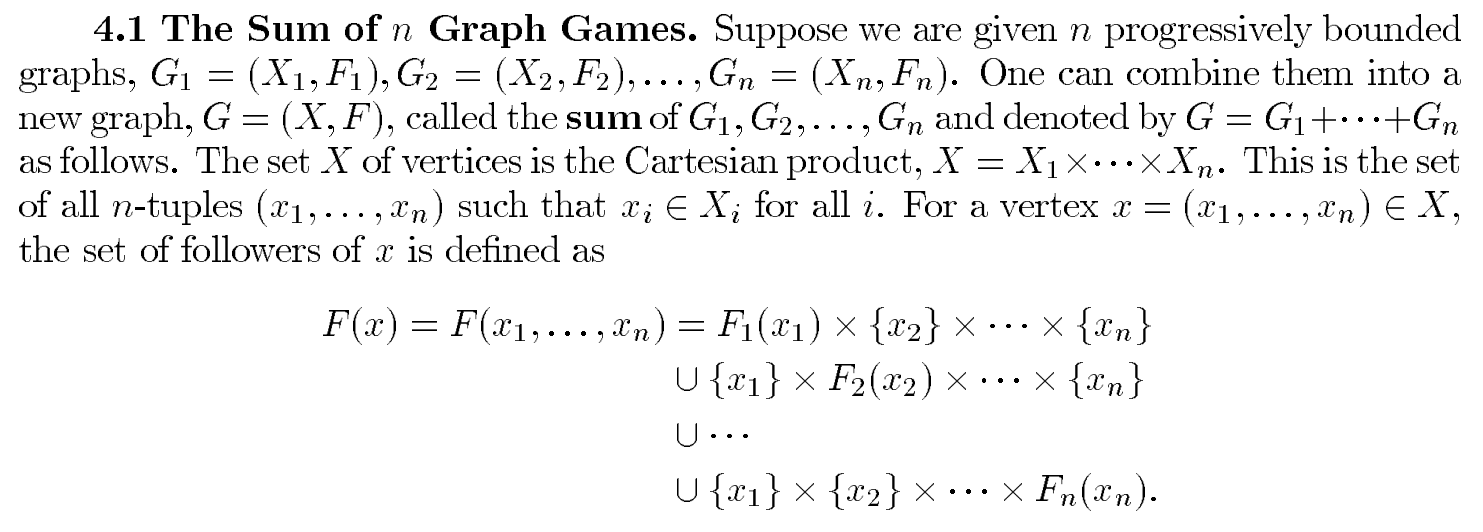
\includegraphics[width=0.5\textwidth,height=0.5\textheight,keepaspectratio]{sumgraph}
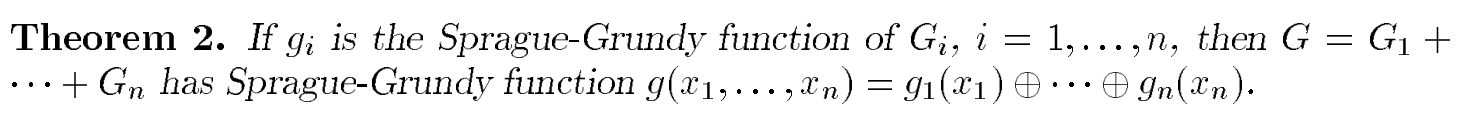
\includegraphics[width=0.5\textwidth,height=0.5\textheight,keepaspectratio]{sgth}
\textbf{Thus}, if a position is a \textbf{N} position, we can cleverly see which position should we go to (what move of a component game to take) such that we reach \textbf {P} position.
\subsection{Mobius}
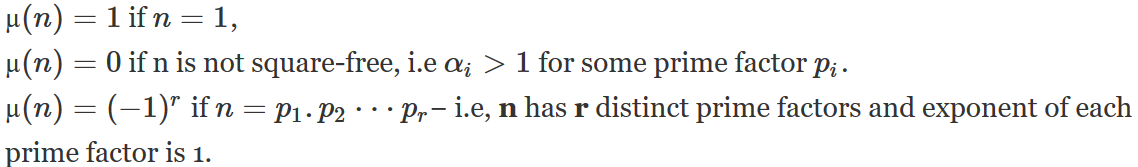
\includegraphics[width=0.5\textwidth,height=0.5\textheight,keepaspectratio]{mob0}
\\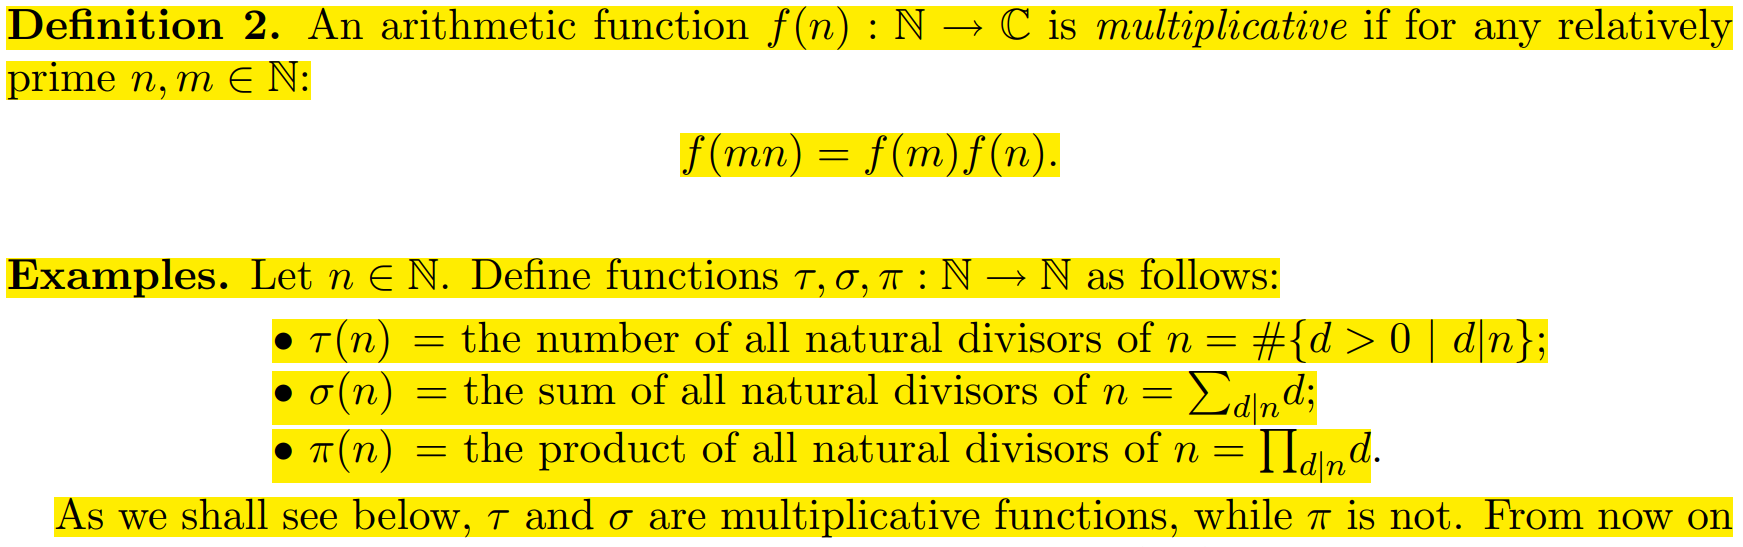
\includegraphics[width=0.5\textwidth,height=0.5\textheight,keepaspectratio]{mob1}
\\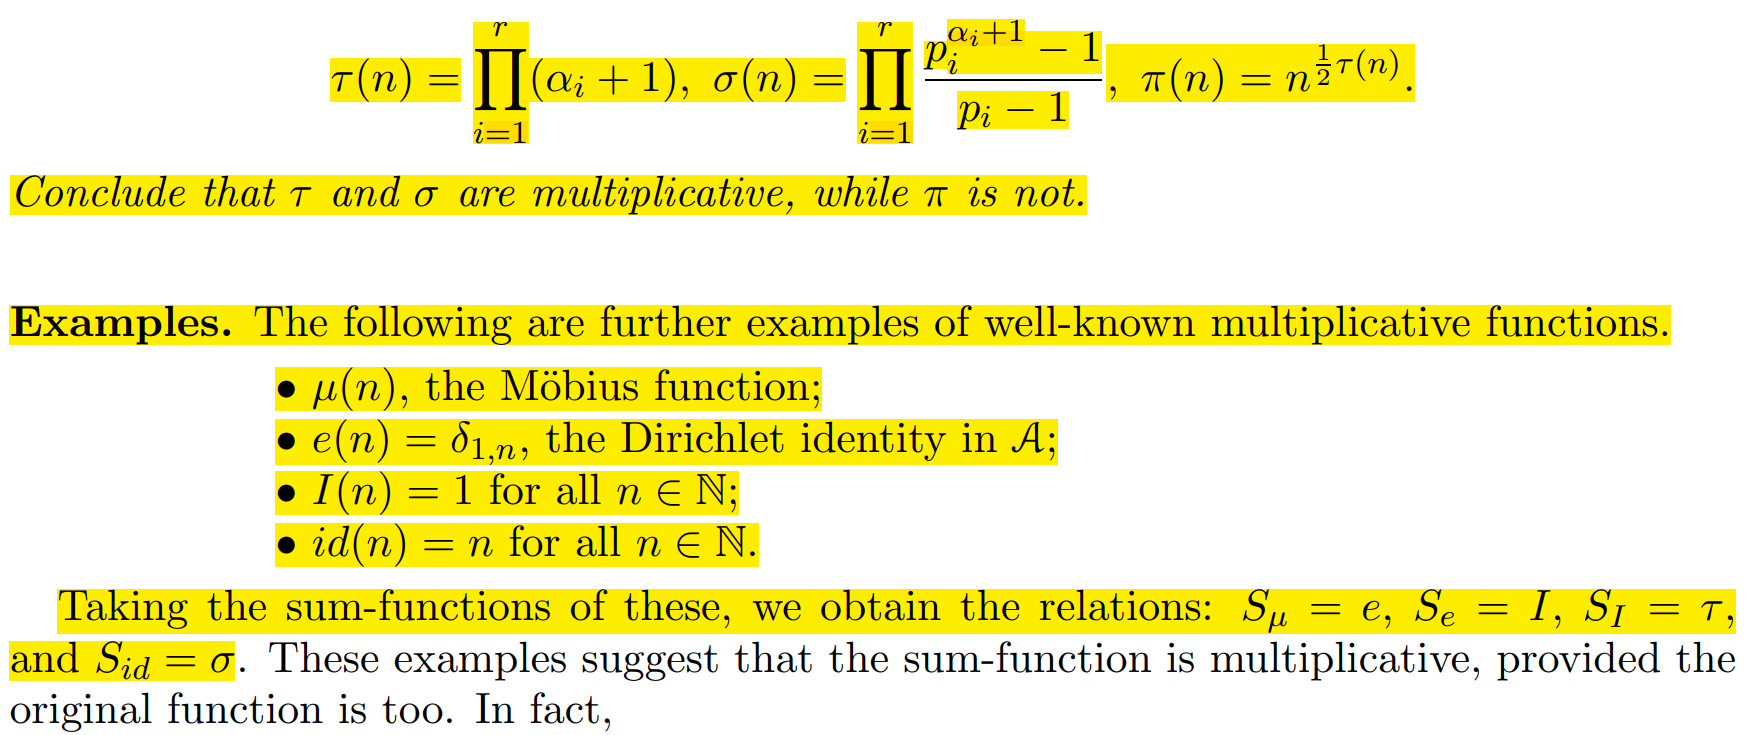
\includegraphics[width=0.5\textwidth,height=0.5\textheight,keepaspectratio]{mob2}
\\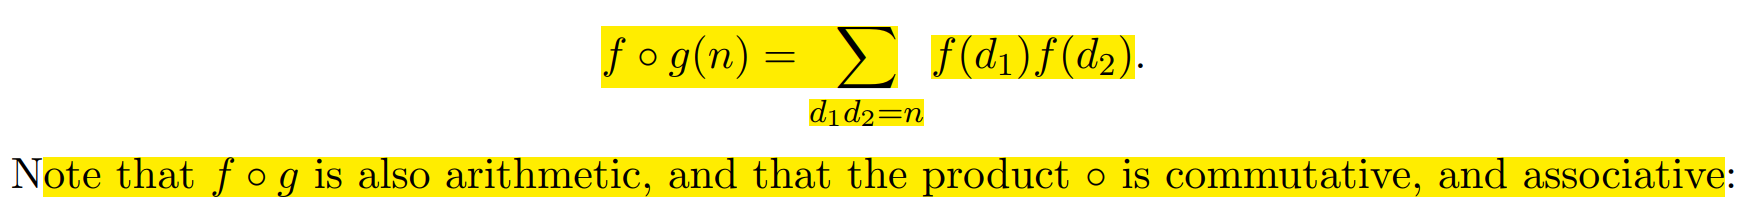
\includegraphics[width=0.5\textwidth,height=0.5\textheight,keepaspectratio]{mob3}
\\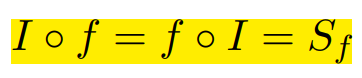
\includegraphics[width=0.1\textwidth,height=0.1\textheight,keepaspectratio]{mob4}
\\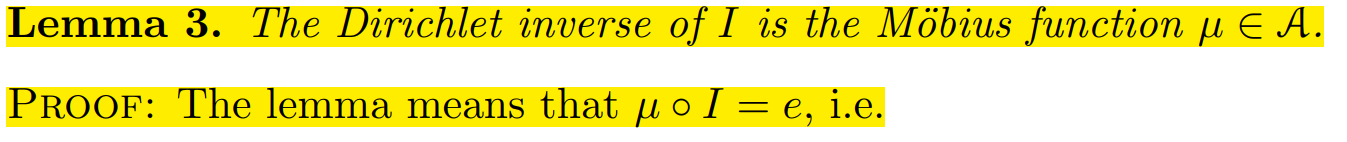
\includegraphics[width=0.5\textwidth,height=0.5\textheight,keepaspectratio]{mob5}
\\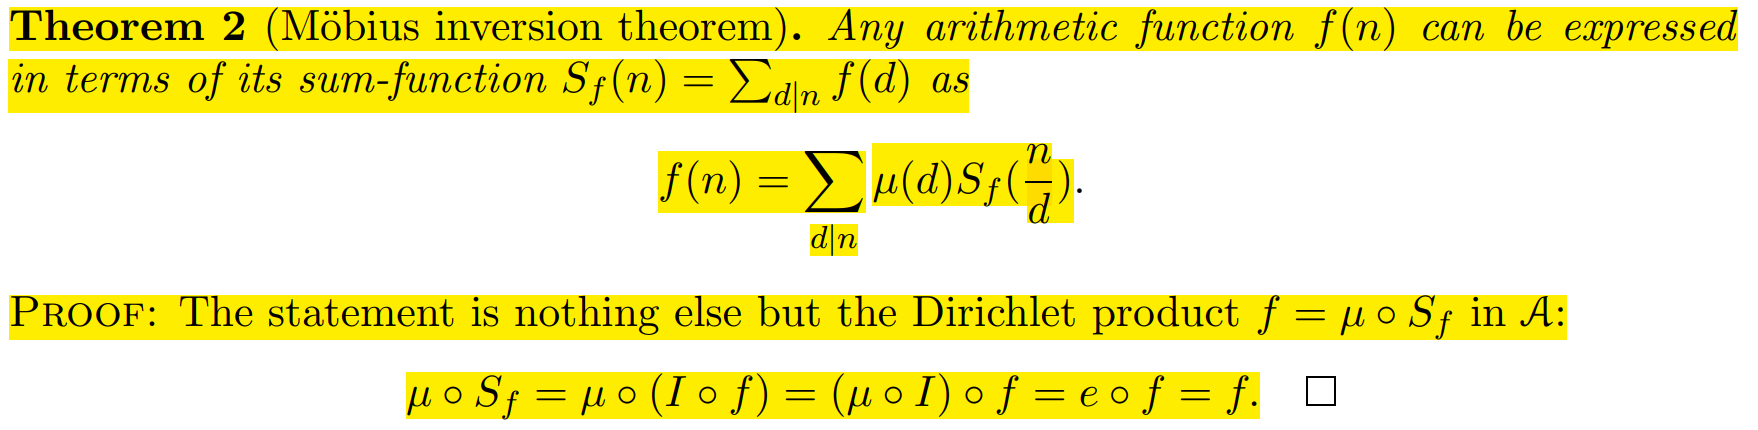
\includegraphics[width=0.5\textwidth,height=0.5\textheight,keepaspectratio]{mob6}
\\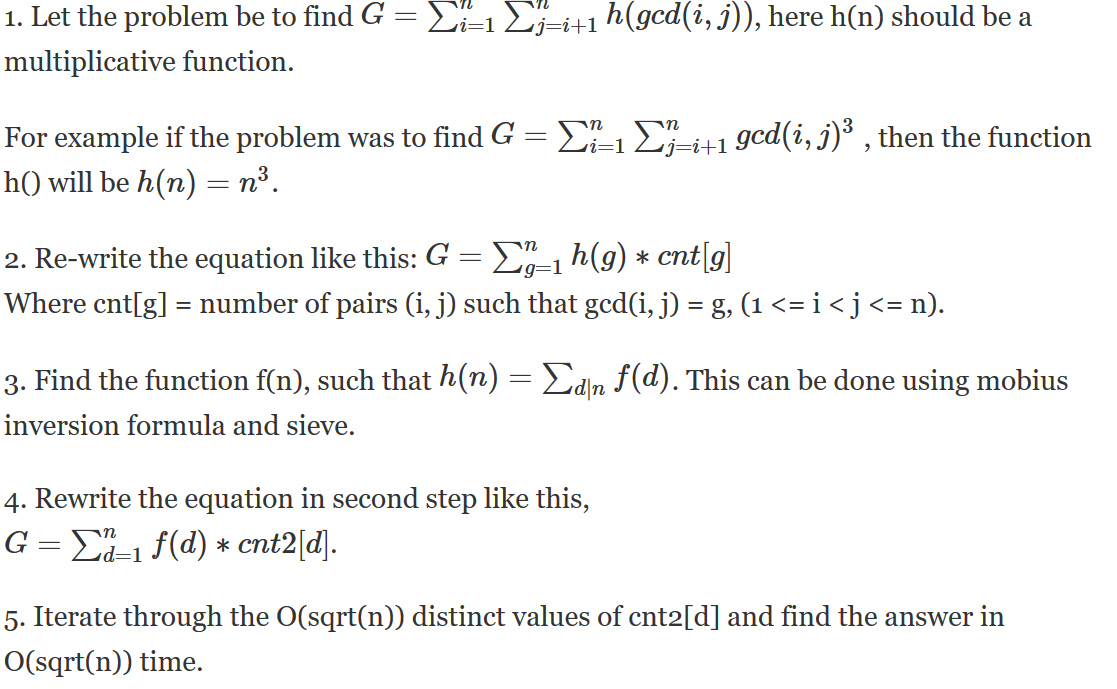
\includegraphics[width=0.5\textwidth,height=0.5\textheight,keepaspectratio]{mob7}
\\$S_{\phi}(n) = id(n)$
$\mu \circ id = \phi (n)$
\begin{minted}{cpp}
for (int i = 1; i <= N; i++) { 
    for (int j = i; j <= N; j += i) {
        f[j] += h[i] * mu[j/i];
    } 
}
\end{minted}
$\sum_{g = 1}^{i}h(g)*cnt[g]$ where $cnt[g] = $ no. of arrays with $gcd(a_1, a_2, a_3, ..., a_n) = g$ and where each $a_k \leq i$. Now $h(g) = $ Dirichlet identity function. Thus it is $\mu \circ e = \mu$. Ans thus we get $\sum_{d = 1}^{i}\mu(d)*f(d)$ where $f(d)$ is the number of arrays with elements in range $[1, i]$ such that $gcd(a_1, \dots, a_n)$ is divisible by $j$. Obviously $f(j) = (\lfloor i/j \rfloor)^n$.
\subsection{Burnside}
The following is the soln of that circle problem
\\n rotational axis and n axis of symmetry 
\\for rotation: rotation by 0 cells, by 1 cell, by 2 cells, etc, by $(n-1)$ cells
\\Now lets apply the lemma, and find the number of stripes that are fixed by the rotation by K cells. If a stripe becomes itself after rotating by K cells, then its 1st cell must have the same color as its (1+K modulo n)-th cell, which is in turn the same as its (1+2K modulo n)-th cell, etc, until we get back to the 1st cell when $m*K \mod n=0$. One may notice that this will happen when $m=n/gcd(K,n)$, thus these must have same color. and we independent choice for $n/(n/gcd(K, n)) = gcd(K, n)$.
\\for axis of symmetry:
\\if (n is even) then we have 
    \\$(n/2)$ axis of symmetry which pass through 2 elements, and for those 2 elements we have independent choice = $3^2$ and for remaining, we get a pair, i.e. $3^{(n - 2)/2}$. Thus total is $3^{(n + 2)/2}$
    \\$(n/2)$ axis of symmetry which passes through non of the elements and again we get a pair, thus $3^{n/2}$ 
if (n is odd) then all n axis of symmetry pass through a single element and we get independent choice for that one element, and for others we get pair i.e. $3 * 3^{(n - 1)/2}$
\\Stirling no. of second kind obey the recurrence $$\stirling{n + 1}{k} = k * \stirling{n}{k} + \stirling{n}{k - 1} \forall n, k > 0$$ where $\stirling{0}{0} = 1$, $\stirling{n}{0} = \stirling{0}{n} = 0$
\\$\frac{1}{k!}\sum_{j=0}^{k}(-1)^{k-j}\binom{k}{j}j^n$
\\$\stirling{n}{k}$ is the number of partitions of \{1, 2, 3, ..., n\} into exactly k parts. 
\subsubsection{Inclusion Exclusion Principle}
$$\left|\bigcup_{i=1}^n A_i \right| = \sum_{\emptyset \neq J\subseteq \{1,2,\ldots ,n\}} (-1)^{|J|-1}{\Biggl |}\bigcap_{j\in J}A_{j}{\Biggr |}$$
$$|\bigcap_{i = 1}^n A_{i}^c| = total - |\bigcap_{i = 1}^n A_i|$$
\subsection{Modulo}
$(a + b) mod m = (a mod m + b mod m) mod m$\\
$.........................-...............$\\
$.........................*...............$\\
\begin{minted}{cpp}
const int m1 = (int) 1e9 + 7;
template <typename T>
inline T add(T a, T b) {
    a += b;
    if (a >= m1) a -= m1;
    return a;
}
template <typename T>
inline T sub(T a, T b) {
    a -= b;
    if (a < 0) a += m1;
    return a;
}

template <typename T>
inline T mul(T a, T b) {
    return (T) (((long long) a * b) % m1);
}

template <typename T>
inline T power(T a, T b) {
    int res = 1;
    while (b > 0) {
        if (b & 1) {
            res = mul<T>(res, a);
        }
        a = mul<T>(a, a);
        b >>= 1;
    }
    return res;
}

template <typename T>
inline T inv(T a) {
    return power<T>(a, m1 - 2);
}
\end{minted}
\subsection{Prob and Comb}
\begin{itemize}
    \item $E[X] = \sum E(X|A_i)P(A_i)$
    \item \href {https://codeforces.com/contest/908/problem/D}{k, $p_a$, $p_b$ prob}, \href {https://github.com/sourabh2311/Competitive-Programming/blob/master/CF/Good%20Bye%202017/D.cpp}{Sol}, if $n + m \geq k \rightarrow p_b(i + j) + p_a*p_b*(i + j + 1) + p_a^2*p_b*(i + j + 2)\dots = (i + j) + \frac{p_a}{p_b}$ Also
    \begin{eqnarray}
    dp[0][0] & = & p_a * dp[1][0] + p_b * dp[0][0]\\
             & = & p_a * dp[1][0] / (1 - p_b)\\
             & = & dp[1][0]
    \end{eqnarray}
    \item \textbf{Dearrangement of n objects}
    \\ $n! * \sum_{k = 0}^n (-1)^k / {k!} =\text{ } !n$
    \\ $!n = (n - 1) * [!(n - 1) + !(n - 2)] \text{ for n }\geq 2$
    \item \textbf{Gambler ruin's problem: }Probability that first player (p for each step) wins. $(1 - (q/p)^{n_1})/(1 - (q/p)^{n_1 + n_2})$. $n_1 = \lceil ev_1/d \rceil$, $n_2 = \lceil ev_2/d \rceil$. In case $p = q = 1/2$, formula is $n_1/(n_1 + n_2)$.
    \item \href{}{UVA 10491}, $ans = (N_{cows} / (N_{cows} + N_{cars})) * (N_{cars} / (N_{cows} + N_{cars} - N_{shows} - 1)) + (N_{cars} / (N_{cows} + N_{cars})) * ((N_{cars} - 1) / (N_{cows} + N_{cars} - N_{shows} - 1))$
    \item $\binom{n}{r} = \binom{n - 1}{r - 1} + \binom{n - 1}{r}$
    \item $\binom{n}{r} = n / r * \binom{n - 1}{r - 1}$
    \item $\sum_{r = 0}^n \binom{n}{r} = 2^n$
    \item $\sum_{m = 0}^n \binom{m}{r} = \binom{n + 1}{r + 1}$
    \item $\sum_{k = 0}^m \binom{n + k}{k} = \binom{n + m - 1}{m}$
    \item $\sum_{i = 0}^n \binom{n}{i}^2 = \binom{2n}{n}$
\end{itemize}
\subsection{Euler's Totient Function}
Also known as phi-function $\phi (n)$, counts the number of integers between 1 and $n$ inclusive, which are coprime to $n$.
\\If $p$ is prime $\phi (p) = p - 1.$
\\If $p$ is a prime number and $k \ge 1$, then there are exactly $p^k / p$ numbers between $1$ and $p^k$ that are divisible by $p$. Which gives us:$\phi(p^k) = p^k - p^{k-1}.$
\\If $a$ and $b$ are relatively prime, then: $\phi(a b) = \phi(a) \cdot \phi(b).$ This relation is not trivial to see. It follows from the Chinese remainder theorem.
\\In general, for not coprime $a$ and $b$, the equation $$\phi(ab) = \phi(a) \cdot \phi(b) \cdot \dfrac{d}{\phi(d)}$$ with $d = \gcd(a, b)$ holds.\\
$ \phi (n) = \phi ({p_1}^{a_1}) \cdot \phi ({p_2}^{a_2}) \cdots \phi ({p_k}^{a_k})$\\
$ = \left({p_1}^{a_1} - {p_1}^{a_1 - 1}\right) \cdot \left({p_2}^{a_2} - {p_2}^{a_2 - 1}\right) \cdots \left({p_k}^{a_k} - {p_k}^{a_k - 1}\right)$\\
$ = p_1^{a_1} \cdot \left(1 - \frac{1}{p_1}\right) \cdot p_2^{a_2} \cdot \left(1 - \frac{1}{p_2}\right) \cdots p_k^{a_k} \cdot \left(1 - \frac{1}{p_k}\right)$ \\ 
$= n \cdot \left(1 - \frac{1}{p_1}\right) \cdot \left(1 - \frac{1}{p_2}\right) \cdots \left(1 - \frac{1}{p_k}\right) $\\
\textbf{Eulers Theorem: }\\
$$a^{\phi(m)} \equiv 1 \pmod m$$ if $a$ and $m$ are relatively prime.

In the particular case when $m$ is prime, Euler's theorem turns into Fermat's little theorem: $$a^{m - 1} \equiv 1 \pmod m$$
\\Converse of euler theorem is also true i.e. if $a^{\phi(m)} \equiv 1 (\mod m)$ then a and m must be coprime.
\subsection{Catalan}
$Cat(n) = \binom{2n}{n} / (n + 1)$
\\$Cat(m) = (2m*(2m - 1)/(m*(m + 1))) * Cat(m - 1)$
\\$Cat(n) = $\begin{enumerate}
    \item the number of ways a convex polygon with n+2 sides can be cut into n triangles
    \item the number of ways to use n rectangles to tile a stairstep shape (1, 2, ..., $n−1$, n).
    \item No. of expressions containing n pairs of parentheses which are correctly matched.
    \item the number of planar binary trees with n+1 leaves
    \item No. of distinct binary trees with n vertices
    \item No. of different ways in which n + 1 factors can be completely parenthesized. Like for \{a, b, c, d\}, one parenthing will be ((ab)c)d.
    \item the number of monotonic paths of length 2n through an n-by-n grid that do not rise above the main diagonal
    \item n pair of people on circle can do non cross hand shakes. i.e. no of ways to connect the 2n points on a circle to form n disjoint chords
    \item no. of permutations of length n that can be stack sorted
    \item no. of non crossing partitions of a set of n elements
\end{enumerate}
\textbf{Note: }Its better to use bigint for catalan computations. Also no. of binary trees with n labelled nodes $= cat[n] * fact[n]$
\subsection{Floyd Cycle Finding}
\begin{minted}{cpp}
// mu = start of the cycle
// lam = its length
// O (mu + lam) time complexity
// O (1) space complexity
ii floydCycleFinding(int x0) {
    // 1st part: finding k * lam
    int tortoise = f(x0), hare = f (f (x0));
    // hare moves at twice speed
    while (tortoise != hare) {
        tortoise = f (tortoise); hare = f(f(hare));
    }
    // thus tor = x_i; hare = x_2i
    // i.e. x_2i = x_{i + k * lam}
    // i.e. k * lam = i.
    // Now if hare is set to beginning
    // i.e. hare = x_0, tor = x_i
    // thus if both now move same no. of steps and in between they become equal, i.e.
    // x_l = x_{i + l}
    // i.e. x_l = x_{l + k * lam}
    // Thus l must be the minimum index and therefore l = mu
    int mu = 0;
    hare = x0;
    while (tortoise != hare) {
        tortoise = f (tortoise); hare = f(hare); mu++
    }
    // finding lam
    int lam = 1; hare = f (tortoise);
    while (tortoise != hare) {
        hare = f (hare); lambda++;
    }
    return ii (mu, lambda);
}
\end{minted}
\subsection{Base Conversion}
\begin{minted}{cpp}
// decimal no. to some base
stack<int> S;
while (q) {
    s.push (q % b);
    q /= b;
}
while (!s.empty ()) {
    cout << process (s.top ()) << " ";
    s.pop ();
}
// base to decimal no.
ll baseToDec () {
    ll ret = 0;
    for (auto &c : num) {
        ret = (ret * base + (c - 48)); // can take mod if final answer is required in mod
    }
    return ret;
}
\end{minted}
\subsection{Extended Euclid}
$ax + by = c$ this is called diophantine eqn and is solvable only when $d = gcd(a, b)$ divides c. so first solve $ax + by = d$ then multiply x, y with $c / d$. Also once we have found a particular soln to this eqn then their exist infinite solns of the form $(x0 + (b/d)*n, y0 - (a/d)*n)$ where n is any integer, note that these infinite solutions are as well the solution to original diophantine eqn. Assume we found the coefs (x1, y1) for (b, a mod b) $\rightarrow$ $b*x1 + (a\text{ mod }b)y1 = g\\ \rightarrow b*x1 + (a - \lfloor(a/b)\rfloor*b)*y1=g\\
\rightarrow a*y1 + b*(x1 - \lfloor (a/b)\rfloor * y1) = g\\
\rightarrow x = y1\text{ \& }y = x1 - \lfloor (a/b)\rfloor*y1$
\begin{minted}{cpp}
void extendedEuclid(int a, int b) {
   if (b == 0) { x = 1; y = 0; d = a; return; } // base case
   extendedEuclid(b, a % b); // similar as the original gcd
   int x1 = y;
   int y1 = x - (a / b) * y;
   x = x1;
   y = y1;
}
\end{minted}
Prob: To find the soln with minimum value of $x + y$ and obviously there has to be range of x, y. Sol: Now $x + y = x_0 + y_0 + n * (b/d - a/d)$. If $a < b$, select smallest possible value of n. If $a > b$ select the largest. And if $a = b$, all solutions have same sum of $x + y$
\subsection{Linear Congruence Equation}
$$a \cdot x = b \pmod n,$$

where $a$, $b$ and $n$ are given integers and $x$ is an unknown integer.

Let us first consider a simpler case where $a$ and $n$ are coprime ($\gcd(a, n) = 1$). 
$$x = b \cdot a ^ {- 1} \pmod n$$
Now consider the case where $a$ and $n$ are not coprime ($\gcd(a, n) \ne 1$). Then the solution will not always exist.

Let $g = \gcd(a, n)$, i.e. the greatest common divisor of $a$ and $n$ (which in this case is greater than one).

Then, if $b$ is not divisible by $g$, there is no solution. 

If $g$ divides $b$, then by dividing both sides of the equation by $g$ (i.e. dividing $a$, $b$ and $n$ by $g$), we receive a new equation:

$$a^\prime \cdot x = b^\prime \pmod{n^\prime}$$

in which $a^\prime$ and $n^\prime$ are already relatively prime, and we have already learned how to handle such an equation. We get $x^\prime$ as solution for $x$.

It can be shown that the original equation has exactly $g$ solutions, and they will look like this:

$$x_i = (x^\prime + i\cdot n^\prime) \pmod n \quad \text{for } i = 0 \ldots g-1$$
\subsection{Sieve}
\begin{minted}{cpp}
ll _sieve_size; // ll is defined as: typedef long long ll;
bitset<10000010> bs; // 10^7 should be enough for most cases
vi primes; // compact list of primes in form of vector<int>
void sieve(ll upperbound) { // create list of primes in [0..upperbound]
   _sieve_size = upperbound + 1; // add 1 to include upperbound
   bs.set(); // set all bits to 1
   bs[0] = bs[1] = 0; // except index 0 and 1
   for (ll i = 2; i <= _sieve_size; i++) if (bs[i]) {
// cross out multiples of i starting from i * i!
           for (ll j = i * i; j <= _sieve_size; j += i) bs[j] = 0;
           primes.push_back((int)i); // add this prime to the list of primes
       } } // call this method in main method
bool isPrime(ll N) { // a good enough deterministic prime tester
    // O(#primes < sqrt(N))
    // O(sqrt(N)/ln(sqrt(N)))
   if (N <= _sieve_size) return bs[N]; // O(1) for small primes
   for (int i = 0; i < (int)primes.size(); i++)
       if (N % primes[i] == 0) return false;
   return true; // it takes longer time if N is a large prime!
} // note: only work for N <= (last prime in vi "primes")^2

vi primeFactors(ll N) { // remember: vi is vector<int>, ll is long long
   vi factors;
   ll PF_idx = 0, PF = primes[PF_idx]; // primes has been populated by sieve
   while (PF * PF <= N) { // stop at sqrt(N); N can get smaller
       while (N % PF == 0) { N /= PF; factors.push_back(PF); } // remove PF
       PF = primes[++PF_idx]; // only consider primes!
   }
   if (N != 1) factors.push_back(N); // special case if N is a prime
   return factors; // if N does not fit in 32-bit integer and is a prime
} // then ‘factors’ will have to be changed to vector<ll>


memset(numDiffPF, 0, sizeof numDiffPF);
//Modified Sieve.
void pre() {
   for (int i = 2; i < MAX_N; i++)
       if (numDiffPF[i] == 0) // i is a prime number
           for (int j = i; j < MAX_N; j += i)
               numDiffPF[j]++; // increase the values of multiples of i
}
// Bottom up euler totient function
for (int i = 0; i <= limit; i++) eu[i] = i;
for (int i = 2; i <= limit; i++) {
    if (eu[i] == i) {
        for (int j = i; j <= limit; j += i) {
            eu[j] -= eu[j] / i;
        }
    }
}
\end{minted}
\subsection{Matrix}
To explain how gaussian elimination allows the computation of the determinant of a square matrix, we should know
\begin{itemize}
    \item Swapping two rows multiplies the determinant by -1
    \item Multiplying a row by a non zero scalar multiplies the determinant by same scalar
    \item Adding to one row a scalar multiple of another does not change the determinant
\end{itemize}
So if d is the product of scalar by which determinant has been multiplied having matrix in row echelon form, we have $det(A) = (\prod diag(B))/d$
\\To find inverse of the matrix augment it with identity matrix and get it RREF, if left block is identity matrix $\rightarrow$ right block is inverse. 
\subsection{Frac lib and Eqn solving}
\begin{minted}{cpp}
struct Frac {
    long long a, b;
    Frac() {
        a = 0, b = 1;
    }
    Frac(int x, int y) {
        a = x, b = y;
        reduce(); ///So we are always reducing out fractions...
    }
    Frac operator+(const Frac &y) {
        long long ta, tb;
        tb = this->b/gcd(this->b, y.b)*y.b;
        ta = this->a*(tb/this->b) + y.a*(tb/y.b);
        Frac z(ta, tb);
        return z;
    }
    Frac operator-(const Frac &y) {
        long long ta, tb;
        tb = this->b/gcd(this->b, y.b)*y.b;
        ta = this->a*(tb/this->b) - y.a*(tb/y.b);
        Frac z(ta, tb);
        return z;
    }
    Frac operator*(const Frac &y) {
        long long tx, ty, tz, tw, g;
        tx = this->a, ty = y.b;
        g = gcd(tx, ty), tx /= g, ty /= g;
        tz = this->b, tw = y.a;
        g = gcd(tz, tw), tz /= g, tw /= g;
        Frac z(tx*tw, ty*tz);
        return z;
    }
    Frac operator/(const Frac &y) {
        long long tx, ty, tz, tw, g;
        tx = this->a, ty = y.a;
        g = gcd(tx, ty), tx /= g, ty /= g;
        tz = this->b, tw = y.b;
        g = gcd(tz, tw), tz /= g, tw /= g;
        Frac z(tx*tw, ty*tz);
        return z;
    }
    bool operator == (const Frac &other) const {
        return a == other.a and b == other.b;
    }
    bool operator < (const Frac &other) const {
        if (a != other.a) return a < other.a;
        else return b > other.b;
    }
    static long long gcd(long long x, long long y) {
        return y == 0 ? x : gcd (y, x % y);
    }
    void reduce() {
        if (a == 0) {  // to handle case when b == 0 (not required in this problem) a = inf (so as to have same ground)
            b = 1;
            return;
        } else {
            long long g = gcd(abs(a), abs(b));
            a /= g, b /= g;
            if(b < 0)   a *= -1, b *= -1;
        }
    }

};
ostream& operator<<(ostream& out, const Frac&x) {
    out << x.a;
    if(x.b != 1)
        out << '/' << x.b;
    return out;
}
int main() { // UVA 10109
    int n, m, i, j, k, N;
    char NUM[100], first = 0;
    long long X, Y;
    Frac matrix[100][100];
    while(scanf("%d", &N) == 1 && N) {
        // m is the number of equations and n is the number of unknowns
        scanf("%d %d", &n, &m);
        for(i = 0; i < m; i++) {
            for(j = 0; j <= n; j++) {
                scanf("%s", NUM);
                if(sscanf(NUM, "%lld/%lld", &X, &Y) == 2) {
                    matrix[i][j].a = X;
                    matrix[i][j].b = Y;
                } else
                    sscanf(NUM, "%lld", &matrix[i][j].a), matrix[i][j].b = 1;
            }
        }
        Frac tmp, one(1,1);
        int idx = 0, rank = 0;
        for(i = 0; i < m; i++) {
            while(idx < n) {
                int ch = -1;
                for(j = i; j < m; j++)
                    if(matrix[j][idx].a) {  // found a non zero element pivot.
                        ch = j;
                        break;
                    }
                if(ch == -1) { // this if condition executes if all the elements in desired column and below the i-1 th row are zero so we need to go to the next column...
                    idx++;
                    continue;
                }
                if(i != ch) // So if the desired pivot element is zero we swap that row with
                    // the closest row that has non zero pivot...
                    for(j = idx; j <= n; j++)
                        swap(matrix[ch][j], matrix[i][j]);
                break;
            }
            if(idx >= n) break;
            tmp = one/matrix[i][idx];
            rank++;
            for(j = idx; j <= n; j++)
                matrix[i][j] = matrix[i][j]*tmp; // So here we are making pivot element 1.
            for(j = 0; j < m; j++) {
                if(i == j)  continue; // This condition executes means that we are ignoring the
                ///pivot row...
                tmp = matrix[j][idx];
                for(k = idx; k <= n; k++) {
                    matrix[j][k] = matrix[j][k] - tmp*matrix[i][k];///Thus now we are making
                    ///all the elements below and above pivot as zero..
                }
            }
            idx++;
        }
        if(first)   puts("");
        first = 1;
        printf("Solution for Matrix System # %d\n", N);
        int sol = 0;
        for(i = 0; i < m; i++) {
            for(j = 0; j < n; j++) {
                if(matrix[i][j].a)
                    break;
            }
            if(j == n) {
                if(matrix[i][n].a == 0 && sol != 1)
                    sol = 0; // INFINITELY
                else
                    sol = 1; // No Solution.
            }
        }
        if(rank == n && sol == 0) {
            for(i = 0; i < n; i++) {
                printf("x[%d] = ", i+1);
                cout << matrix[i][n] << endl;
            }
            continue;
        }
        if(sol == 1)
            puts("No Solution.");
        else
            printf("Infinitely many solutions containing %d arbitrary constants.\n", n-rank);
    }
    return 0;
}
\end{minted}
\subsection{Finding Power Of Factorial Divisor}
You are given two numbers $n$ and $k$. Find the largest power of $k$ (say $x$) such that $n!$ is divisible by $k^x$.
\subsubsection{Prime $k$}
$$\Bigl\lfloor\dfrac{n}{k}\Bigr\rfloor + \Bigl\lfloor\dfrac{n}{k^2}\Bigr\rfloor + \ldots + \Bigl\lfloor\dfrac{n}{k^i}\Bigr\rfloor + \ldots$$
Implementation:
\begin{minted}{cpp}
int fact_pow (int n, int k) {
	int res = 0;
	while (n) {
		n /= k;
		res += n;
	}
	return res;
}
\end{minted}
\subsubsection{Composite $k$}

The same idea can't be applied directly. Instead we can factor $k$, representing it as $k = k_1^{p_1} \cdot \ldots \cdot k_m^{p_m}$. For each $k_i$, we find the number of times it is present in $n!$ using the algorithm described above - let's call this value $a_i$. The answer for composite $k$ will be

$$\min_ {i=1 \ldots m} \dfrac{a_i}{p_i}$$
\subsection{GCD, LCM}
\begin{minted}{cpp}
    // time complexity O(log(min(a, b) / gcd(a, b)))
    int gcd (int a, int b) { return b == 0 ? a : gcd (b, a % b); }
    int lcm (int a, int b) { return a * (b / gcd (a, b)); }
\end{minted}
\begin{itemize}
    \item For a series of numbers if you want next no. to have gcd 1 with all previous no. then $GCD(a_j, LCM(a_1, a_2, \dots, a_{j - 1})) = 1$.
    \item if $p|N \& p|M$ then $p|gcd(N, M)$ as $N = pk, M = pl \rightarrow$ N, M have p common so gcd will also have p.
    \item $N|P \& M|P \rightarrow lcm(N, M)|P$.
    \item $N = gcd(N, m) \Leftrightarrow N|M$
    \item $M = lcm(N, M) \Leftrightarrow N|M$
    \item $gcd(P*N, P*M) = P*gcd(N, M)$
    \item $lcm(P*N, P*M) = P*lcm(N, M)$
    \item If $gcd(N_1, N_2) = 1$ then $gcd(N_1 * N_2, M) = gcd(N_1, M) * gcd(N_2, M)$ and $lcm(N_1*N_2, M) = lcm(N_1, M)*lcm(N_2, M)/M$
    \item gcd(gcd(N, M), P) = gcd(N, gcd(M, P))
    \item lcm(lcm(N, M), P) = lcm(N, lcm(M, P))
    \item gcd(M, N, P) = gcd(gcd(M, N), P) = gcd(M, gcd(N, P))
    \item lcm(M, N, P) = lcm(lcm(M, N), P) = lcm(M, lcm(N, P))
    \item for integers $N_1, \dots, N_k$ and $k \geq 2$, 
    $$lcm(gcd(N_1, M), gcd(N_2, M), \dots, gcd(N_k, M)) = gcd(lcm(N_1, \dots, N_k), M)$$
    $$gcd(lcm(N_1, M), lcm(N_2, M), \dots, lcm(N_k, M)) = lcm(gcd(N_1, \dots, N_k), M)$$
\end{itemize}
\subsection{Some properties of Fibonacci numbers}
\begin{itemize}
    \item $F_0 = 0, F_1 = 1, F_n = F_{n-1} + F_{n-2}$
    \item Cassini's identity: $F_{n-1} F_{n+1} - F_n^2 = (-1)^n$
    \item The "addition" rule: $F_{n+k} = F_k F_{n+1} + F_{k-1} F_n$
    \item Applying the previous identity to the case $k = n$, we get: $F_{2n} = F_n (F_{n+1} + F_{n-1})$
    \item From this we can prove by induction that for any positive integer $k$, $F_{nk}$ is multiple of $F_n$.
    The inverse is also true: if $F_m$ is multiple of $F_n$, then $m$ is multiple of $n$.
    \item GCD identity: $GCD(F_m, F_n) = F_{GCD(m, n)}$
    \item Every positive integer can be expressed uniquely as a sum of fibonacci numbers such that no two numbers are equal or consecutive fibonacci numbers. This can be done greedily by taking the highest fibonacci no. at each point.
    \item Fibonacci nos are periodic under modulo. The period of the fibonacci sequence modula a positive integer j is the smallest positive integer m such that such that $F_m \equiv 0 (mod j) \& F_{m + 1} \equiv 1 (mod j)$
    \item \[\begin{bmatrix}
    1 & 1\\
    1 & 0
    \end{bmatrix}^{\!p}
=
\begin{bmatrix}
    fib(p + 1) & fib (p)\\
    fib (p) & fib (p - 1)
    \end{bmatrix}
    \]
    \textit{Thus higher fibs can be computed in $O(\log{p})$}
    \item $$F_n = \frac{\left(\frac{1 + \sqrt{5}}{2}\right)^n - \left(\frac{1 - \sqrt{5}}{2}\right)^n}{\sqrt{5}}$$
    \item You can immediately notice that the second term's absolute value is always less than $1$, and it also decreases very rapidly (exponentially). Hence the value of the first term alone is "almost" $F_n$. This can be written strictly as:
    $$F_n = \left[\frac{\left(\frac{1 + \sqrt{5}}{2}\right)^n}{\sqrt{5}}\right]$$
\end{itemize}
\subsection{Wilson Theorem}
States that for a prime no. p, $(p - 1)! \mod p = p - 1$.
\\Note that $n! \mod p$ is 0 if $n \geq p$. Suppose p is prime and is close to input number n. For example $25! \mod 29$. From wilson theorem, we know that $28! \mod 29 = -1 \equiv 28$, so we basically need to find $(28 * inverse(28, 29) * inverse (27, 29) * inverse (26, 29)) \mod 29$
\\Time complexity $O((p - n) * \log n)$
\subsection{Factorial modulo $p$ in $O(p \log n)$}
all divisors of p are 1, find mod p.
\begin{minted}{cpp}
int factmod(int n, int p) {
	int res = 1;
	while (n > 1) {
		res = (res * ((n/p) % 2 ?  p-1 : 1)) % p;
		for (int i = 2; i <= n%p; ++i)
			res = (res * i) % p;
		n /= p;
	}
	return res % p;
}
\end{minted}
This implementation works in $O(p \log_p n)$.
\subsection{Modular Inverse}
For an arbitrary (but coprime) modulus $m$: $a ^ {\phi (m) - 1} \equiv a ^{-1} \mod m$\\
For a prime modulus $m$: $a ^ {m - 2} \equiv a ^ {-1} \mod m$
\begin{minted}{cpp}
inv[1] = 1;
for(int i = 2; i < m; ++i)
    inv[i] = (m - (m/i) * inv[m%i] % m) % m;
\end{minted}
\textbf{Binomial coeff modulo large prime no}
\begin{minted}{cpp}
fact[0] = 1;
for (int i = 1; i <= maxn; i++) {
    fact[i] = (fact[i - 1] * (i % m)) % m;
}
// afterwards we can compute binomial coeff in O(log m)
ll getC(int n, int k) {
    ll res = fact[n];
    ll div = fact[k] * fact[n - k] % m;
    div = pow (div, m - 2, m);
    return (res * div) % m;
}
\end{minted}
\textbf{Binomial Coeff modulo prime power}
let $g(x) := \frac{x!}{p^{c(x)}}$. Then we can write the binomial coefficient as: $$\binom n k = \frac {g(n) p^{c(n)}} {g(k) p^{c(k)} g(n-k) p^{c(n-k)}} = \frac {g(n)} {g(k) g(n-k)}p^{c(n) - c(k) - c(n-k)}$$

Now $g(x)$ is now free from the prime divisor $p$. Therefore $g(x)$ is coprime to m, and we can compute the modular inverses of $g(k)$ and $g(n-k)$.

Notice, if $c(n) - c(k) - c(n-k) \ge b$, than $p^b | p^{c(n) - c(k) - c(n-k)}$, and the binomial coefficient is $0$.
\subsection{Gray Code}
000, 001, 011, 010, 110, 111, 101, 100, so $G(4) = 6$.
\begin{minted}{cpp}
int g (int n) {
    return n ^ (n >> 1);
}
\end{minted}
\subsubsection{Finding inverse gray code}
Given Gray code $g$, restore the original number $n$.
\\The easiest way to write it in code is:
\begin{minted}{cpp}
int rev_g (int g) {
  int n = 0;
  for (; g; g >>= 1)
    n ^= g;
  return n;
}
\end{minted}
\subsection{Discrete Logarithm}
The discrete logarithm is an integer $x$ solving the equation

$a^x \equiv b \pmod m$

where $a$ and $m$ are relatively prime. 

$O(\sqrt{m} \log m)$
\subsubsection{Algorithm}
Let $x = np - q$

Obviously, any value of $x$ in the interval $[0; m)$ can be represented in this form, where $p \in [1; \lceil \frac{m}{n} \rceil ]$ and $q \in [0; n]$.

$a^{np} \equiv ba^q \pmod m$


$n = m/n$
\subsubsection{Implementation}
\begin{minted}{cpp}
int solve (int a, int b, int m) {
	int n = (int) sqrt (m + .0) + 1;
 
	int an = 1;
	for (int i=0; i<n; ++i)
		an = (an * a) % m;
 
	map<int,int> vals;
	for (int i=1, cur=an; i<=n; ++i) {
		if (!vals.count(cur))
			vals[cur] = i;
		cur = (cur * an) % m;
	}
 
	for (int i=0, cur=b; i<=n; ++i) {
		if (vals.count(cur)) {
			int ans = vals[cur] * n - i;
			if (ans < m)
				return ans;
		}
		cur = (cur * a) % m;
	}
	return -1;
}
\end{minted}
\subsection{Chinese Remainder Theorem}
\begin{minted}{cpp}
#include<bits/stdc++.h>
using namespace std;
const int N = 20;
long long GCD(long long a, long long b) { return (b == 0) ? a : GCD(b, a % b); }
inline long long LCM(long long a, long long b) { return a / GCD(a, b) * b; }
inline long long normalize(long long x, long long mod) { x %= mod; if (x < 0) x += mod; return x; }
struct GCD_type { long long x, y, d; };
GCD_type ex_GCD(long long a, long long b)
{
    if (b == 0) return {1, 0, a};
    GCD_type pom = ex_GCD(b, a % b);
    return {pom.y, pom.x - a / b * pom.y, pom.d};
}
int testCases;
int t;
long long a[N], n[N], ans, lcm;
int main()
{
    ios_base::sync_with_stdio(0);
    cin.tie(0);
    cin >> t;
    for(int i = 1; i <= t; i++) cin >> a[i] >> n[i], normalize(a[i], n[i]);
    ans = a[1];
    lcm = n[1];
    for(int i = 2; i <= t; i++)
    {
        auto pom = ex_GCD(lcm, n[i]);
        int x1 = pom.x;
        int d = pom.d;
        if((a[i] - ans) % d != 0) return cerr << "No solutions" << endl, 0;
        ans = normalize(ans + x1 * (a[i] - ans) / d % (n[i] / d) * lcm, lcm * n[i] / d);
        lcm = LCM(lcm, n[i]); // you can save time by replacing above lcm * n[i] /d by lcm = lcm * n[i] / d
    }
    cout << ans << " " << lcm << endl;
 
    return 0;
}
\end{minted}
\subsection{Primitive Root}
\subsubsection{Definition}
$g$ is a primitive root modulo n if and only if for any integer $a$ such that $gcd(a, n) = 1$, there exists an integer $k$ such that:

$g^k \equiv a \pmod n$.

$k$ is then called the index or discrete logarithm of $a$ to the base $g$ modulo $n$. $g$ is also called the generator of the multiplicative group of integers modulo $n$.

\subsubsection{Existence}

Primitive root modulo $n$ exists if and only if:
\begin{itemize}
    \item $n$ is 1, 2, 4, or
    \item $n$ is power of an odd prime number $(n = p^k)$, or
    \item $n$ is twice power of an odd prime number $(n = 2 . p^k)$.
\end{itemize}
\subsubsection{Implementation}
The following code assumes that the modulo p is a prime number. To make it works for any value of p, we must add calculation of $\phi (p)$.
\begin{minted}{cpp}
int generator (int p) {
	vector<int> fact;
	int phi = p-1,  n = phi;
	for (int i=2; i*i<=n; ++i)
		if (n % i == 0) {
			fact.push_back (i);
			while (n % i == 0)
				n /= i;
		}
	if (n > 1)
		fact.push_back (n);
 
	for (int res=2; res<p; ++res) {
		bool ok = true;
		for (size_t i=0; i<fact.size() && ok; ++i)
			ok &= powmod (res, phi / fact[i], p) != 1;
		if (ok)  return res;
	}
	return -1;
}
\end{minted}
\subsection{Discrete Root}

The problem of finding discrete root is defined as follows. Given a prime $n$ and two integers $a$ and $k$, find all $x$ for which:

$x^k \equiv a \pmod n$
\subsubsection{The algorithm}

We will solve this problem by reducing it to the discrete logarithm problem.

Let's apply the concept of a primitive root modulo $n$. Let $g$ be a primitive root modulo $n$. Note that since $n$ is prime, it must exist, and it can be found in $O(Ans \cdot \log \phi (n) \cdot \log n) = O(Ans \cdot \log^2 n)$ plus time of factoring $\phi (n)$.

We can easily discard the case where $a = 0$. In this case, obviously there is only one answer: $x = 0$.

Since we jnow that $n$ is a prime, any number between 1 and $n-1$ can be represented as a power of the primitive root, and we can represent the discrete root problem as follows:

$(g^y)^k \equiv a \pmod n$

where

$x \equiv g^y \pmod n$

This, in turn, can be rewritten as

$(g^k)^y \equiv a \pmod n$

Now we have one unknown $y$, which is a discrete logarithm problem. The solution can be found using Shanks' baby-step-giant-step algorithm in $O(\sqrt {n} \log n)$ (or we can verify that there are no solutions).

Having found one solution $y_0$, one of solutions of discrete root problem will be $x_0 = g^{y_0} \pmod n$.
Finding all solutions from one known solution

To solve the given problem in full, we need to find all solutions knowing one of them: $x_0 = g^{y_0} \pmod n$.

Let's recall the fact that a primitive root always has order of $\phi (n)$, i.e. the smallest power of $g$ which gives 1 is $\phi (n)$. Therefore, if we add the term $\phi (n)$ to the exponential, we still get the same value:

$x^k \equiv g^{ y_0 \cdot k + l \cdot \phi (n)} \equiv a \pmod n \forall l \in Z$

Hence, all the solutions are of the form:

$x = g^{y_0 + \frac {l \cdot \phi (n)}{k}} \pmod n \forall l \in Z$.

where $l$ is chosen such that the fraction must be an integer. For this to be true, the numerator has to be divisible by the least common multiple of $\phi (n)$ and $k$. Remember that least common multiple of two numbers $lcm(a, b) = \frac{a \cdot b}{gcd(a, b)}$; we'll get

$x = g^{y_0 + i \frac {\phi (n)}{gcd(k, \phi (n))}} \pmod n \forall i \in Z$.

This is the final formula for all solutions of discrete root problem.
\subsubsection{Implementation}
\begin{minted}{cpp}
    int delta = phi / gcd (k, phi);
	vector<int> ans;
	for (int cur=any_ans % delta; cur < phi; cur += delta)
		ans.push_back (powmod (g, cur, n));
	sort (ans.begin(), ans.end());
	printf ("%d\n", ans.size());
	for (size_t i=0; i<ans.size(); ++i)
		printf ("%d ", ans[i]);
\end{minted}
\subsection{Josephus Problem}
\subsubsection{For k = 2}
\begin{eqnarray}n & = & 1, 2, 3, 4, 5, 6\\
f(n) & = & 1, 1, 3, 1, 3, 5
\end{eqnarray}
Thm: if $n = 2^m + l$ where $0 \leq l < 2^m$ then $f(n) = 2l + 1$.
\subsubsection{For general $k \geq 1$}
$f(n, k) =  ((f(n - 1, k) + k - 1) \mod n) + 1$ with $f(1, k) = 1$ which takes the simpler form $g(n, k) = (g(n - 1, k) + k) \mod n$ with $g(1, k) = 0$. This approach has running time O(n).
\\Aliter O(klogn)
\begin{eqnarray}
g(n, k) &=& 0 \text{ if n = 1 (because of 0 indexing)}\\
        &=& (g(n - 1, k) + k) \mod n \text{ if $1 < n < k$}\\
        &=& \lfloor k * ((g(n_m, k) - n \mod k) \mod n_m) / (k - 1) \rfloor 
\end{eqnarray}
where $n_m = n - \lfloor n/k \rfloor$ if $k \leq n$
\subsection{Root Solving}
\begin{minted}{cpp}
// Following is the solution for UVA 10428
typedef long long int ll;
const double eps = 1e-7;
struct Polynomial {
    vector<double> coef;
    int deg;
    Polynomial() {}
    Polynomial(int dd) {
        deg = dd;
        coef.resize(deg + 1);
    }
    void fix(Polynomial &given) {
        int dec = 0;
        for (int i = given.deg; i >= 0; i--) {
            if (abs(given.coef[i]) < eps) {
                dec++;
            } else break;
        }
        dec *= -1;
        given.coef.resize(given.deg + dec + 1);
        given.deg += dec;
        return;
    }
    Polynomial operator + (const Polynomial &other) {
        Polynomial ret;
        if (deg > other.deg) {
            ret.deg = deg;
            ret.coef.resize(deg + 1);
            for (int i = deg; i > other.deg; i--) {
                ret.coef[i] = coef[i];
            }
            for (int i = other.deg; i >= 0; i--) {
                ret.coef[i] = coef[i] + other.coef[i];
            }
            fix(ret);
            return ret;
        } else {
            ret.deg = other.deg;
            ret.coef.resize(other.deg + 1);
            for (int i = other.deg; i > deg; i--) {
                ret.coef[i] = other.coef[i];
            }
            for (int i = deg; i >= 0; i--) {
                ret.coef[i] = coef[i] + other.coef[i];
            }
            fix(ret);
            return ret;
        }
    }
    Polynomial operator - (const Polynomial &other) {
        Polynomial ret;
        if (deg > other.deg) {
            ret.deg = deg;
            ret.coef.resize(deg + 1);
            for (int i = deg; i > other.deg; i--) {
                ret.coef[i] = coef[i];
            }
            for (int i = other.deg; i >= 0; i--) {
                ret.coef[i] = coef[i] - other.coef[i];
            }
            fix(ret);
            return ret;
        } else {
            ret.deg = other.deg;
            ret.coef.resize(other.deg + 1);
            for (int i = other.deg; i > deg; i--) {
                ret.coef[i] = other.coef[i];
            }
            for (int i = deg; i >= 0; i--) {
                ret.coef[i] = coef[i] - other.coef[i];
            }
            fix(ret);
            return ret;
        }
    }
    Polynomial operator * (const pair<double, int> u) {
        double d = u.first;
        int dega = u.second;
        Polynomial ret;
        ret.deg = deg + dega;
        ret.coef.assign(ret.deg + 1, 0);
        for (int i = deg; i >= 0; i--) {
            ret.coef[i + dega] = (coef[i] * d);
        }
        fix(ret);
        return ret;
    }
    bool operator != (const Polynomial &other) {
        if (deg != other.deg) return true;
        for (int i = deg; i >= 0; i--) {
            if (coef[i] != other.coef[i]) return true;
        }
        return false;
    }
};
pair<Polynomial, Polynomial> polyDiv(Polynomial &n, Polynomial &d) { // To do n / d
    Polynomial zero;
    zero.deg = 0;
    zero.coef.push_back(0);
    if (n.deg < d.deg) {
        return make_pair(zero, n);
    }
    Polynomial q;
    q.deg = (n.deg);
    q.coef.assign(q.deg + 1, 0);
    Polynomial r = n;
    while (r != zero and r.deg >= d.deg) {
        double t = (r.coef[r.deg] / d.coef[d.deg]);
        q.coef[r.deg - d.deg] += t;
        r = r - d * make_pair(t, r.deg - d.deg);
    }
    q.fix(q); r.fix(r);
    return make_pair(q, r);
}
double f(Polynomial &a, double x) {
    double result = 0;
    for (int i = a.deg; i >= 0; i--) {
        result = result * x + a.coef[i];
    }
    return result;
}
double f_(Polynomial &a, double x) {
    double result = 0;
    for (int i = a.deg; i > 0; i--) {
        result = result * x + a.coef[i] * i;
    }
    return result;
}
double newtonsMethod(Polynomial &a, double x0) {
    double x1 = x0;
    while (true) {
        x0 = x1;
        x1 = x0 - f(a, x0)/f_(a, x0);
        if (abs(x1 - x0) < eps) break;
    }
    return x1;
}
void findRoot(Polynomial a, vector<double> &roots, int n) {
    for (int i = 0; i < n; i++) {
        roots.push_back(newtonsMethod(a, 0));
        Polynomial d(1);
        d.coef[1] = 1;
        d.coef[0] = -roots.back();
        auto u = polyDiv(a, d);
        a = u.first;
    }
}
\end{minted}
\subsection{Integration}
\subsubsection{Simpson rule}
$$x_i = a + i h, ~~ i = 0 \ldots 2n,$$ $$h = \frac {b-a} {2n}.$$
$$\int_a ^ b f (x) dx \approx \left(f (x_0) + 4 f (x_1) + 2 f (x_2) + 4f(x_3) + 2 f(x_4) + \ldots + 4 f(x_{2N-1}) + f(x_{2N}) \right)\frac {h} {3} $$
\begin{minted}{cpp}
const int N = 1000 * 1000; // number of steps (already multiplied by 2)
double simpson_integration(double a, double b){
    double h = (b - a) / N;
    double s = f(a) + f(b); // a = x_0 and b = x_2n
    for (int i = 1; i <= N - 1; ++i) { // Refer to final Simpson's formula
        double x = a + h * i;
        s += f(x) * ((i & 1) ? 4 : 2);
    }
    s *= h / 3;
    return s;
}
\end{minted}
\subsection{Continued Fractions}
\begin{minted}{cpp}
while (n != 1) {
            int q = n / d;
            int r = n % d;
            // in c++ when we divide negative no. with positive no. both quotient and rem are -ve.
            if (n < 0) {
                q--;
                r = r + d;
            }
            ans.push_back(q);
            n = d;
            d = r;
}
\end{minted}
\subsection{Side Notes}
\begin{enumerate}
    \item No. of digits in a no. $n = \lfloor(\log_{10}{n})\rfloor + 1$
    \item No. of digits in $\binom{n}{k} = \lfloor(\sum_{i = n - k + 1}^{n}\log_{10}{i} - \sum_{i = 1}^{k}\log_{10}{i)})\rfloor + 1$
    \item No. of digits of a no. in some base b$ = floor(1 + \log_b{no.} + eps)$. Also make sure that input no. is not 0.
    \item
\begin{minted}{cpp}
// to compute (a * b) mod m when a * b can go above ll
ll bmodm;
ll compute (ll a, ll &b, ll &m) {
    if (a == 1) return bmodm;
    if (a & 1) return (((2 % m) * compute (a / 2, b, m) + bmodm) % m);
    else return ((2 % m) * compute (a/2, b, m)) % m;
}
\end{minted}
\end{enumerate}
\textbf{Prob: }Lenghts from 1 to n, max. no. of triangles?
\\\textbf{Sol: }
\begin{minted}{cpp}
void precal () {
    F[3] = P[3] = 0;
    ll var = 0;
    for (int i = 4; i <= 1000000; i++) {
        if (i % 2 == 0) {
            var++;
        }
        P[i] = P[i - 1] + var;
        F[i] = F[i - 1] + P[i];
    }
    // F[n] has ans
}
            \end{minted}
\section{Graphs}
\subsection{Basic}
\begin{minted}{cpp}
// graph check
void graphcheck (int u) {
    dfs_num[u] = explored;
    for (auto &v : adjlist[u]) {
        if (dfs_num[v] == unvisited) {  // tree edge
            dfs_parent[v] = u;
            graphcheck (v);
        } else if (dfs_num[v] == explored) {  // back edge hence not DAG.
            if (v == dfs_parent[u]) cout << "two ways\n"
            else cout << "back edge\n"
        } else {  // dfs_num[v] == visited
            // forward/cross edge
            // [u [v v] u] this is tree/forward
            // [v [u u] v] back
            // [v v] [u u] cross
        }

    }
}
\end{minted}
\begin{minted}{cpp}
bool dfs(int v) {
    color[v] = 1;
    for (int u : adj[v]) {
        if (color[u] == 0) {
            parent[u] = v;
            if (dfs(u))
                return true;
        } else if (color[u] == 1) {
            cycle_end = v;
            cycle_start = u;
            return true;
        }
    }
    color[v] = 2;
    return false;
}
// if it returns true, follow the parents of cycle_end
\end{minted}
\subsection{Articulation Points and Bridges (undirected graph)}
\begin{minted}{cpp}
/* Variation
A slight variation to this problem is how many disconnected components would result as a direct consequence of removing a vertex u */
void ArticulationPoint(int u)
{
    dfs_num[u] = dfs_low[u] = dfs_num_counter++;
    for(int i = 0; i < adj_list[u].size(); i++)
    {
        int v = adj_list[u][i];
        
        if(dfs_num[v] == -1)
        {
            dfs_parent[v] = u;
            if(u == dfs_root) root_children++;

            ArticulationPoint(v);
            
            // we increment articulation_vertex here
            if(dfs_low[v] >= dfs_num[u])
                articulation_vertex[u]++;
            if (dfs_low[v.first] > dfs_num[u])
                printf(" Edge (%d, %d) is a bridge\n", u, v.first);
                
            dfs_low[u] = min(dfs_low[u], dfs_low[v]);
        }
        else if(v != dfs_parent[u])
            dfs_low[u] = min(dfs_low[u], dfs_num[v]);
    }
}

int main() 
{
    dfs_num_counter = 0;
    // articulation_vertex initialized to 1 here
    articulation_vertex.assign(N, 1);
    for(int i = 0; i < N; i++)
        if (dfs_num[i] == -1)
        {
            dfs_root = i; root_children = 0;
            ArticulationPoint(i);
            // special case for root
            // number of connected components after the removal of root
            // is equal to how many children root has
            articulation_vertex[dfs_root] = root_children;
        }
}
\end{minted}
\subsection{Tree}
\subsubsection{LCA}
\begin{itemize}
    \item Tarjan's offline LCA. for each query (a, b) you should do q[a].pb(b) and q[b].pb(a).
\\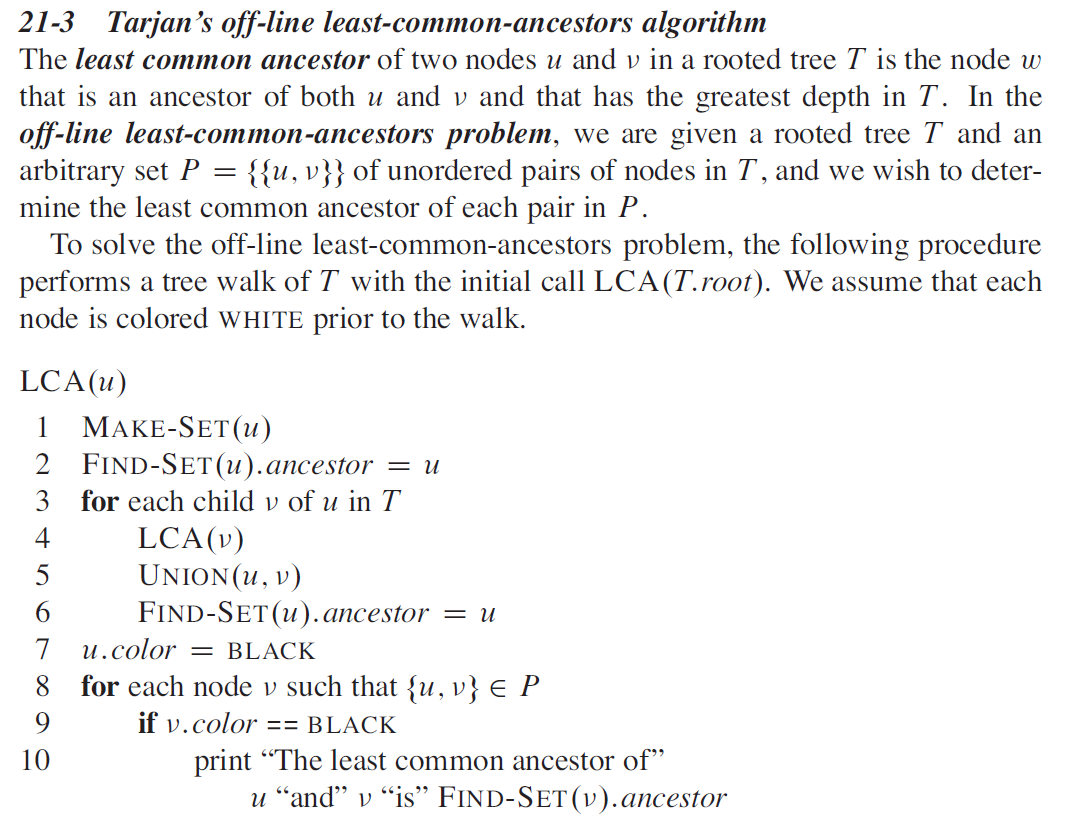
\includegraphics[width=0.5\textwidth,height=0.5\textheight,keepaspectratio]{tar}
\end{itemize}
\subsubsection{Important Problems}
\subsubsection{MVC on Tree}
\begin{minted}{cpp}
int mvc(int at, int flag, int parent) { //You can start this from any node, i.e. in main: int ans =  min(mvc(0, 0, -1), mvc(0, 1, -1)); and handle the case n == 1 seperately
   if(memo[at][flag] != -1) {
       return memo[at][flag];
   }
   if(glist[at].size() == 1 and parent != -1) { //leaf node
       return memo[at][flag] = flag;
   }
   int ans = flag;
   if(flag) // to take this
   {
       for(auto to : glist[at]) {
           if(to != parent)
               ans += min(mvc(to, 0, at), mvc(to, 1, at));
       }
   } else { //we must take its neighbours
       for(auto to : glist[at]) {
           if(to != parent)
               ans += mvc(to, 1, at);
       }
   }
   return memo[at][flag] = ans;
}  // Similar code can be written to find MWIS.
\end{minted}
\subsection{Bipartite Matching}
\subsubsection{Hopcroft Karp}
\begin{minted}{cpp}
#define FOR(i, a, b) for (int i = a; i <= b; i++)
#define REP(i, n) for (int i = 0; i < n; i++)
int n, m, matchX[maxN], matchY[maxN];
int dist[maxN];
vector<int> adj[maxN];
bool Free[maxN];
bool bfs() {
    queue<int> Q;
    FOR (i, 1, n)
        if (!matchX[i]) {  // only free vertices are pushed in queue and have their distance set to 0. Thus already matched vertices in X will have their distance set to INF.
            dist[i] = 0;
            Q.push(i);
        }
        else dist[i] = INF;
    dist[0] = INF;  // 0 is nil
    // Thus we would always start from free vertices traverse then alternating path and if in end from Y there is no match i.e. its a free vertice, we found an augmenting path.
    // Side Notes: If we popped an already matched vertex from queue then it wont go to its matching edges neighbor as its matchY is popped vertex itself and hence it wont have distance set to INF.
    while (!Q.empty()) {
        int i = Q.front(); Q.pop();
        REP(k, adj[i].size()) {
            int j = adj[i][k];
            if (dist[matchY[j]] == INF) {
                dist[matchY[j]] = dist[i] + 1;
                Q.push(matchY[j]);
            }
        }
    }
    return dist[0] != INF;
}
bool dfs(int i) {
    if (!i) return true; // to handle nil.
    REP(k, adj[i].size()) {
        int j = adj[i][k];
        if (dist[matchY[j]] == dist[i] + 1 && dfs(matchY[j])) {
            matchX[i] = j;
            matchY[j] = i;
            return true;
        }
    }
    dist[i] = INF;
    return false;
}
int hopcroft_karp() {
    int matching = 0;
    while (bfs())
        FOR (i, 1, n)
            if (!matchX[i] && dfs(i))
                matching++;
    return matching;
}
void dfs_konig(int i) {
    Free[i] = false;
    REP(k, adj[i].size()) {
        int j = adj[i][k];
        if (matchY[j] && matchY[j] != INF) {
            int x = matchY[j];
            matchY[j] = INF;  // as we have undirected edge, we dont want to traverse that same edge again, so its just a way of noting that.
            if (Free[x]) dfs_konig(x);
        }
    }
}
void solve() {
    printf("%d", hopcroft_karp());
    FOR (i, 1, n)
        if (!matchX[i])
            dfs_konig(i);  // finding Z.
    FOR (i, 1, n)
        if (matchX[i] && Free[i])  // i.e. in L but not in Z.
            printf(" r%d", i);
    FOR (j, 1, m)
        if (matchY[j] == INF)  // i.e. we traversed this edge i.e. its in R intersection Z.
            printf(" c%d", j);
    putchar('\n');
}
void initialize() {
    FOR (i, 1, n) {
        adj[i].clear();
        matchX[i] = 0;
        Free[i] = true;
    }
    memset(matchY, 0, (m + 1) * sizeof(int));
}
int ar[5];
char buff[20];
void read_line() {
    gets(buff);
    int len = strlen(buff), i = 0, m = 0;
    while (i < len)
        if (buff[i] != ' ') {
            ar[m] = 0;
            while (i < len && buff[i] != ' ')
                ar[m] = ar[m] * 10 + buff[i++] - 48;
            m++;
        }
        else i++;
}
main() {
    int k, u, v;
    while (scanf(" %d %d %d ", &n, &m, &k) != EOF) {
        if (!n && !m && !k) break;
        initialize();
        while (k--) {
            read_line();
            adj[ar[0]].pb(ar[1]);
        }
        solve();
    }
}
\end{minted}
\subsubsection{Using max flow algo}
Our MM problem can be reduced to max flow problem by assigning a dummy source vertex s connected to all vertices in set 1 and all vertices in set 2 are connected to dummy sink vertex t. The edges are directed (s to u, u to v, v to t) where u belongs to set 1 and v belongs to set 2). Set capacities of all edges in this flow graph to 1.
\subsection{Paths}
\begin{minted}{cpp}
// Code to find euler tour (will be able to find euler path provided we start with correct vertex) for an undirected graph.
list<int> cyc; // we need list for fast insertion in the middle
void EulerTour(list<int>::iterator i, int u) {
    for (int j = 0; j < (int)AdjList[u].size(); j++) {
        ii v = AdjList[u][j];
        if (v.second) { // if this edge can still be used/not removed
            v.second = 0; // make the weight of this edge to be 0 (‘removed’)
            for (int k = 0; k < (int)AdjList[v.first].size(); k++) {
                ii uu = AdjList[v.first][k]; // remove bi-directional edge
                if (uu.first == u && uu.second) {
                    uu.second = 0;
                    break;
                } 
            }
            EulerTour(cyc.insert(i, u), v.first);
        } 
    }
}
// inside int main()
cyc.clear();
EulerTour(cyc.begin(), A); // cyc contains an Euler tour starting at A
for (list<int>::iterator it = cyc.begin(); it != cyc.end(); it++)
    printf("%d\n", *it); // the Euler tour
\end{minted}
\subsubsection{No. of paths}
\begin{itemize}
    \item No. of paths of length L, from a to b is stored in $M^L[a][b]$. $m_{i, j} = 1$ if there is an edge from i to j. This would work even in case of multiple edges if some pair of vertices (i, j) is connected with m edges then we can record this in the adjacency matrix by setting M[i][j] = m. Also this would work if the graph contains loops 
    \item No. of shortest paths of fixed length: We are given a directed weighted graph G, G[i][j] = weight of an edge (i, j) and is equal to infinity if there is no edge for each pair of vertices (i, j) we have to find the length of the shortest path between i and j that consists of exactly k edges. $$L_{k + 1}[i][j] = min_{p = 1, \dots, n}(L_k[i][p] + G[p][j])$$
\end{itemize}
\subsection{SCC}
\subsubsection{Tarjan}
\begin{minted}{cpp}
vi dfs_num, dfs_low, S, visited; // global variables
void tarjanSCC(int u) {
    dfs_low[u] = dfs_num[u] = dfsNumberCounter++; // dfs_low[u] <= dfs_num[u]
    S.push_back(u); // stores u in a vector based on order of visitation
    visited[u] = 1;
    for (int j = 0; j < (int)AdjList[u].size(); j++) {
        ii v = AdjList[u][j];
        if (dfs_num[v.first] == UNVISITED)
            tarjanSCC(v.first);
        if (visited[v.first]) // condition for update
            dfs_low[u] = min(dfs_low[u], dfs_low[v.first]); 
    }
    if (dfs_low[u] == dfs_num[u]) { // if this is a root (start) of an SCC
        printf("SCC %d:", ++numSCC); // this part is done after recursion
        while (1) {
            int v = S.back(); S.pop_back(); visited[v] = 0;
            printf(" %d", v);
            if (u == v) break; 
        }
        printf("\n");
    } 
}
// inside int main()
dfs_num.assign(V, UNVISITED); dfs_low.assign(V, 0); visited.assign(V, 0);
dfsNumberCounter = numSCC = 0;
for (int i = 0; i < V; i++)
    if (dfs_num[i] == UNVISITED)
        tarjanSCC(i);
\end{minted}
\subsubsection{Kosaraju}
\begin{minted}{cpp}
vector < vector<int> > g, gr;
vector<bool> used;
vector<int> order, component;
void dfs1 (int v) {
    used[v] = true;
    for (size_t i=0; i<g[v].size(); ++i)
        if (!used[ g[v][i] ])
            dfs1 (g[v][i]);
    order.push_back (v);
}
void dfs2 (int v) {
    used[v] = true;
    component.push_back (v);
    for (size_t i=0; i<gr[v].size(); ++i)
        if (!used[ gr[v][i] ])
            dfs2 (gr[v][i]);
}
int main() {
    ... reading n ...
    for (;;) {
        int a, b;
        ... reading next edge (a,b) ...
        g[a].push_back (b);
        gr[b].push_back (a);
    }
    used.assign (n, false);
    for (int i=0; i<n; ++i)
        if (!used[i])
            dfs1 (i);
    used.assign (n, false);
    for (int i=0; i<n; ++i) {
        int v = order[n-1-i];
        if (!used[v]) {
            dfs2 (v);
            ... printing next component ...
            component.clear();
        }
    }
}
\end{minted}
\subsection{DAG}
\subsubsection{Min Path cover on DAG}
This is described as a problem of finding the min. no. of paths to cover each vertex on DAG. The start of each path can be arbitrary, we are just interested in min. no. of paths.
\\Construct a bipartite graph $G' = (V_{out} \cup V_{in}, E')$ from G where $V_{out/in} = \{v \in V: v \text{ has poitive out/in degree}\}$
\\$E' = \{(u, v) \in (V_{out}, V_{in}) : (u, v) \in E\}$
\\G' is a bipartite graph, do max. matching on it. Say answer obtained is m that means ans is $|V| - m$ as initially |V| vertices can be convered with |V| paths of length of length 0 (the vertices themselves). One matching b/w vertex a and b using edge (a, b) says that we can use one less path as edge (a, b) in E' can cover path $a \in V_{out} \& b\in V_{in}$
\subsection{APSP Floyd Warshalls}
\begin{minted}{cpp}
for (int k = 0; k < V; k++) {
    for (int i = 0; i < V; i++) {
        for (int j = 0; j < V; j++) {
            if (adjmat[i][j] > adjmat[i][k] + adjmat[k][j]) {
                adjmat[i][j] = adjmat[i][k] + adjmat[k][j];
                path[i][j] = path[k][j];
            }
        }
    }
}
\end{minted}
\subsection{MST (Kruskal)}
\begin{minted}{cpp}
// O (ElogV)
// Connected, undirected weighted graph
vector<pair<int, ii> > edgelist;
for (int i = 0; i < E; i++) {
    cin >> u >> v >> w;
    edgelist.pb (make_pair(w, ii (u, v)));
}
sort(edgelist.begin (), edgelist.end ());
int mstCost = 0;
UFDS uf (V);
for (int i = 0; i < E and uf.numSets > 1; i++) {
    auto front = edgelist[i];
    if (!uf.isSameSet (front.second.first, front.second.second)) {
        mstCost += front.first;
        uf.unionSet (front.second.first, front.second.second);
    }
}
cout << mstCost;
\end{minted}
\subsection{SSSP}
\subsubsection{Dijkstra}
\begin{minted}{cpp}
// Subpaths of shortest paths from u to v are shortest paths
// This implementation would work even if the graph has negative edge provided there is no negative cycle
// O(ElogV)
struct node {
    int cost, vertex;
    node () {}
    node (int n, int c) {
        vertex = n; cost = c;
    }
    bool operator < (const node &node) const {
        return cost > node.cost;  // as priority queue is max heap
    }
}
int dijkstra (int s, int e) {
    memset (dist, inf, sizeof (dist));
    dist[s] = 0;
    priority_queue<node> pq;
    pq.push (node (s, 0));
    int from, to, wt, cost;
    while (!pq.empty ()) {
        from = pq.top ().vertex;
        cost = pq.top ().cost;
        pq.pop ();
        if (from == e) return dist[e];
        if (cost == dist[from]) {  // lazily deleting
            for (int i = 0; i < adjlist[from].size (); i++) {
                to = adjlist[form][i].first;
                wt = adjlist[from][i].second;
                if (dist[to] > dist[from] + wt) {
                    dist[to] = dist[from] + wt;
                    p[to] = from;
                    pq.push (node (to, dist[to])); }}}}}
\end{minted}
\subsubsection{Bellman ford}
\begin{minted}{cpp} 
// For negative edge weights provided we have no negative cycles.
// Idea: Shortest path must have atmost |V| - 1 edges.
// Thus if we relax each each edge |V| - 1 times then we would have got the answer as in first relaxation edge(start, neighbour) will be correct and so on...
vi dist (V, inf);
dist[s] = 0;
bool modified = true;
for (int i = 0; i < V - 1 and modified; i++) {
    modified = false;
    for (int u = 0; u < V; u++) {
        for (int j = 0; j < adjlist[u].size (); j++) {
            ii v = adjlist[u][j];
            if (dist[v.first] > dist[u] + v.second) {
                dist[v.first] = dist[u] + v.second;
                p[v.first] = u;
                modified = true;
            }
        }
    }
}
\end{minted}
\subsection{Max Flow}
\subsubsection{Edmond karps}
\begin{minted}{cpp}
// O (V * E^2)
void augment(int v, int minEdge) { // traverse BFS spanning tree from s->t
    if (v == s) { f = minEdge; return; } // record minEdge in a global var f
    else if (p[v] != -1) { augment(p[v], min(minEdge, res[p[v]][v]));
    res[p[v]][v] -= f; res[v][p[v]] += f; }
}
    // in main
    mf = 0; // mf stands for max_flow
    while (1) { // O(VE^2) (actually O(V^3 E) Edmonds Karp’s algorithm
        f = 0;
        // run BFS
        vi dist(MAX_V, INF); dist[s] = 0; queue<int> q; q.push(s);
        p.assign(MAX_V, -1); // record the BFS spanning tree, from s to t!
        while (!q.empty()) {
            int u = q.front(); q.pop();
            if (u == t) break; // immediately stop BFS if we already reach sink t
            for (int v = 0; v < MAX_V; v++) // note: this part is slow
                if (res[u][v] > 0 && dist[v] == INF)
                    dist[v] = dist[u] + 1, q.push(v), p[v] = u; // 3 lines in 1!
        }
        augment(t, INF); // find the min edge weight ‘f’ in this path, if any
        if (f == 0) break; // we cannot send any more flow (‘f’ = 0), terminate
        mf += f; // we can still send a flow, increase the max flow!
    }
\end{minted}
\begin{itemize}
    \item \textbf{MWIS on a bipartite graph}
    \\Problem is equivalent to finding the minimum weight vertex cover in the graph. The latter can be solved using maximum flow techniques:
    \\Introduce a super-source S and a super-sink T. connect the nodes on the left side of the bipartite graph to S, via edges that have their weight as capacity. Do the same thing for the right side and sink T. Assign infinite capacity to the edges of the original graph.

    Now find the minimum S-T cut in the constructed network. The value of the cut is the weight of the minimum vertex cover. 

    Thus, to actually reconstruct the vertex cover, just collect all the vertices that are adjacent to cut edges, or alternatively, the left-side nodes not reachable from S and the right-side nodes reachable from S.
\end{itemize}
\subsection{Minimum Cost Flow}
\begin{minted}{cpp}
    while(true) {
            vector<long long int> dist(n + 1, INF);
            dist[0] = 0;
            p.assign(n + 1, -1);
            for(int i = 0; i < n; i++) {
                for(int u = 0; u <= n; u++) {
                    for(auto to : glist[u]) {
                        if(flow[to][u] > 0 && dist[u] - mat[to][u].cost < dist[to]) {
                            dist[to] = dist[u] - mat[to][u].cost;
                            p[to] = u;
                        }
                        else if(mat[u][to].cap - flow[u][to] > 0 && dist[u] + mat[u][to].cost < dist[to]) {
                            dist[to] = dist[u] + mat[u][to].cost;
                            p[to] = u; }}}}
            if(dist[n] == INF) break;
            augment(n, INF);
            if(f == 0) break;
            mf += f;
            mincost += dist[n] * f;
        }
        if(mf == totransfer)
            cout << mincost << "\n";
\end{minted}
\subsection{Kirchhoff's matrix tree theorem}
Problem: You are given a connected undirected graph (with possible multiple edges) represented using an adjacency matrix. Find the number of different spanning trees of this graph.
\\Let $A$ be the adjacency matrix of the graph: $A_{u,v}$ is the number of edges between $u$ and $v$. Let $D$ be the degree matrix of the graph: a diagonal matrix with $D_{u,u}$ being the degree of vertex $u$ (including multiple edges and loops - edges which connect vertex $u$ with itself).
The Laplacian matrix of the graph is defined as $L = D - A$. According to Kirchhoff's theorem, all cofactors of this matrix are equal to each other, and they are equal to the number of spanning trees of the graph. The $(i,j)$ cofactor of a matrix is the product of $(-1)^{i + j}$ with the determinant of the matrix that you get after removing the $i$-th row and $j$-th column.\\ Thus we can get answer in $O(n^3)$.
\subsection{Counting Labeled graphs}
\subsubsection{Labeled graphs}
$$G_n = 2^{\frac{n(n-1)}{2}}$$
\subsubsection{Connected labeled graphs}
$$C_n = G_n - \frac{1}{n} \sum_{k=1}^{n-1} k \binom{n}{k} C_k G_{n-k}$$
\subsubsection{Labeled graphs with $k$ connected components}
$$D[n][k] = \sum_{s=1}^{n} \binom{n-1}{s-1} C_s D[n-s][k-1]$$
\subsection{Heavy Light Decomposition}
\begin{minted}{cpp}
    void hld(int v, int pr = -1){
  chain[v] = cnt - 1; // what chain does this vertex belong to, cnt is initiallized to 1.
  num[v] = all++; // seemingly, ordering will be like, contiguous one will be belonging to same chain, all is initiallized to 0.
  if(!csz[cnt - 1]) { // if the size of this chain is 0, make top vertex of this chain as 'v'
    top[cnt - 1] = v;
  }
  ++csz[cnt - 1]; // what size is of this chain
  if(nxt[v] != -1){
    hld(nxt[v], v);
  }
  forn(i, g[v].size()){
    int to = g[v][i];
    if(to == pr || to == nxt[v]){
      continue;
    }
    ++cnt; // next chain
    hld(to, v);
  }
}

ll go(int a, int b){
  ll res = 0;
  while(chain[a] != chain[b]){
    if(depth[top[chain[a]]] < depth[top[chain[b]]]) swap(a, b);
    int start = top[chain[a]];
    if(num[a] == num[start] + csz[chain[a]] - 1) // alone else part should be enough
      res = max(res, mx[chain[a]]);
    else
      res = max(res, go(1, 0, n - 1, num[start], num[a]));
    a = p[start];
  }
  if(depth[a] > depth[b]) swap(a, b);
  res = max(res, go(1, 0, n - 1, num[a], num[b]));
  return res;
}
\end{minted}
\section{Some Basic}
\begin{minted}{cpp}
#pragma GCC optimize("Ofast")  // tells the compiler to optimize the code for speed to make it as fast as possible (and not look for space)
#pragma GCC optimize ("unroll-loops")  // normally if we have a loop there is a "++i" instruction somewhere. We normally dont care because code inside the loop requires much more time but in this case there is only one instruction inside the loop so we want the compiler to optimize this.
#pragma GCC target("sse,sse2,sse3,ssse3,sse4,popcnt,abm,mmx,avx,tune=native")  // tell the compiler that our cpu has simd instructions and allow him to vectorize our code
\end{minted}
\begin{minted}{cpp}
// generating lexicographic next combination better than k while loops
bool next_combination(vector<int>& a, int n) {
    int k = (int)a.size();
    for (int i = k - 1; i >= 0; i--) {
        if (a[i] < n - k + i + 1) {
            a[i]++;
            for (int j = i + 1; j < k; j++)
                a[j] = a[j - 1] + 1;
            return true;
        }
    }
    return false;
}
\end{minted}
\begin{minted}{cpp}
// Tell the minimum no. of intervals to cover the entire big interval.
void solve() {
    // Greedy Algorithm
    sort (data.begin (), data.end ()); 
    for (; i < data.size(); i = j) {
       if (data[i].first > rightmost) break;
       for (j = i + 1; j < data.size() and data[j].first <= rightmost; j++) {
           if (data[j].second > data[i].second) {
               i = j;
           }
       }
       ans.push_back(data[i]);
       rightmost = data[i].second;
       if (rightmost >= m) break;

    }
    if (rightmost < m) {
       cout << "0\n";
    }
}
\end{minted}
\begin{minted}{cpp}
// Parity of $n -$ no. of cycles = parity of inversions.
for (int i = 1; i <= n; i++) {  // 1 indexed
    if (was[i]) continue;
    cyc++;
    int p = i;
    while (!was[p]) {
        was[p] = 1;
        p = a[p];
    }
}
\end{minted}
\begin{minted}{cpp}
struct UFDS {
    vector<int> p, rank, setSizes;
    int numSets;
    UFDS(int N) {
        numSets = N;
        rank.assign(N, 0);
        p.assign(N, 0);
        for (int i = 0; i < N; i++)
            p[i] = i;
        setSizes.assign(N, 1);
    }
    int findSet(int i) {
        return (p[i] == i) ? i : p[i] = findSet(p[i]);
    }
    bool isSameSet(int i, int j) {
        return findSet(i) == findSet(j);
    }
    void unionSet(int i, int j) {
        if (!isSameSet(i, j)) {
            int x = findSet(i), y = findSet(j);
            if (rank[x] > rank[y]) {
                setSizes[x] += setSizes[y];
                p[y] = x;
            } else {
                setSizes[y] += setSizes[x];
                p[x] = y;
                if (rank[x] == rank[y])
                    rank[y]++;
            }
            numSets--;
        }
    }
    int setSize(int i) {
        return setSizes[findSet(i)];
    }
    int numDisjointSets() {
        return numSets;
    }
};
\end{minted}
\begin{minted}{cpp}
// max 1d range sum
sum = ans = 0;
finish = -1;
local_start = 0;
for (int i = 0; i < n ;i++) {
    sum += A[i];
    if (sum > ans) {
        ans = sum;
        start = local_start;
        finish = i;
    }
    if (sum < 0) {
        sum = 0;
        local_start = i + 1;
    }
}
// if instead of maximum you want to find minimum, simply negate all terms. As suppose minimum sum is (ak, a_{k + 1}, ..., a_{k + l}) which must be negative and most (maximum in other dirn) negative possible. Thus (-ak,...) is maximum positive possible as suppose there was some other range with maximum possible that means its negative (actual) is more minimum then our current which leads to contradiction
\end{minted}
\begin{minted}{cpp}
// max 2d range sum
// grid need not be square
// O(n^4)
// Commented part shows for torus
cin >> n;
for (int i = 0; i < n; i++) { // < 2n
    for (int j = 0; j < n; j++) { // <2n
        cin >> A[i][j]; 
        /*
        if (i < n and j < n) {
            cin >> A[i][j];
            A[i + n][j] = A[i][j + n] = A[i + n][j + n] = A[i][j];
        }
        */
        if (i) A[i][j] += A[i - 1][j];
        if (j) A[i][j] += A[i][j - 1];
        if (i and j) A[i][j] -= A[i - 1][j - 1];
    }
    int maxSubRect = -127 * 100 * 100;
    for (int i = 0; i < n; i++) {
        for (int j = 0; j < n; j++) {
            for (int k = i; k < n; k++) {  // < i + n
                for (int l = j; l < n; l++) {  // < j + n
                    subRect = A[k][l];
                    if (i) subRect -= A[i - 1][l];
                    if (j) subRect -= A[k][j - 1];
                    if (i and j) subRect += A[i - 1][j - 1];
                    maxSubRect = max (maxSubRect, subRect);
                }
            }
        }
    }
// "No tree" => make tree (1) = -inf
// no tree (0) = 1.
}
\end{minted}
\begin{minted}{cpp}
// O(n^3)
int maxSum2D () {
    int maxsum = INT_MIN, finalleft, finalright, finaltop, finalbottom;
    for (int leftc = 0; leftc < COL; leftc++) {
        vector<int> temp (ROW, 0);
        for (int rightc = leftc; rightc < COL; rightc++) {
            for (int i = 0; i < ROW; i++) {
                temp[i] += M[i][rightc]
            }
            int rstart, rend;
            sum = kadane (temp, rstart, rend);
            // kadane will give us rstart and rend
            if (sum > maxsum) {
                maxsum = sum;
                finalleft = left;
                finalright = right;
                finaltop = rstart;
                finalbottom = rend;
            } 
        }
    }
}
\end{minted}
\begin{minted}{cpp}
int __builtin_clz(int x);// number of leading zero
int __builtin_ctz(int x);// number of trailing zero
int __builtin_clzll(long long x);// number of leading zero
int __builtin_ctzll(long long x);// number of trailing zero
int __builtin_popcount(int x);// number of 1-bits in x
int __builtin_popcountll(long long x);// number of 1-bits in x
lsb(n): (n & -n); // last bit (smallest)
floor(log2(n)): 31 - __builtin_clz(n | 1);
floor(log2(n)): 63 - __builtin_clzll(n | 1);
// Suppose we have a pattern of N bits set to 1 in an integer and we want the next permutation of N 1 bits in a lexicographical sense. For example, if N is 3 and the bit pattern is 00010011, the next patterns would be 00010101, 00010110, 00011001,00011010, 00011100, 00100011, and so forth. The following is a fast way to compute the next permutation.
unsigned int v; // current permutation of bits 
unsigned int w; // next permutation of bits
unsigned int t = v | (v - 1); // t gets v's least significant 0 bits set to 1
// Next set to 1 the most significant bit to change, 
// set to 0 the least significant ones, and add the necessary 1 bits.
w = (t + 1) | (((~t & -~t) - 1) >> (__builtin_ctz(v) + 1));  
\end{minted}
\subsection{To find subarray (contiguous) with maximum average and length more than \textbf{k}}
\begin{minted}{cpp}
// 1) binary search for the average
// This is the code for steps 2-5.
int maxIndexDiff(int arr[], int n) 
{ 
    int maxDiff; 
    int i, j; 
  
    int LMin[n], RMax[n]; 
  
    // Construct LMin[] such that LMin[i] 
    // stores the minimum value 
    // from (arr[0], arr[1], ... arr[i]) 
    LMin[0] = arr[0]; 
    for (i = 1; i < n; ++i) 
        LMin[i] = min(arr[i], LMin[i - 1]); 
  
    // Construct RMax[] such that RMax[j] 
    // stores the maximum value 
    // from (arr[j], arr[j+1], ..arr[n-1]) 
    RMax[n - 1] = arr[n - 1]; 
    for (j = n - 2; j >= 0; --j) 
        RMax[j] = max(arr[j], RMax[j + 1]); 
  
    // Traverse both arrays from left to right 
    // to find optimum j - i 
    // This process is similar to merge() 
    // of MergeSort 
    i = 0, j = 0, maxDiff = -1; 
    while (j < n && i < n) { 
        if (LMin[i] < RMax[j]) { 
            maxDiff = max(maxDiff, j - i); 
            j = j + 1; 
        } 
        else
            i = i + 1; 
    } 
  
    return maxDiff + 1; 
} 
  
// utility Function which subtracts X from all 
// the elements in the array 
void modifyarr(int arr[], int n, int x) 
{ 
    for (int i = 0; i < n; i++) 
        arr[i] = arr[i] - x; 
} 
void calcprefix(int arr[], int n) {
    int s = 0; 
    for (int i = 0; i < n; i++) { 
        s += arr[i]; 
        arr[i] = s;  }}
int longestsubarray(int arr[], int n, int x) {  // main func.
    modifyarr(arr, n, x); 
    calcprefix(arr, n); 
    return maxIndexDiff(arr, n); }
\end{minted}
\subsection{LIS}
\begin{minted}{cpp}
vi getLIS (int ans) {
    vi lis;
    for (int i = n - 1; i >= 0; i--) {
        if (L[i] == ans) {
            lis.pb (sequence[i]);
            ans--;
        }
    }
    reverse (lis.begin (), lis.end ());
    return lis;
}
//------------------------
// O(nlogk) - k is the length of LIS.
int LIS (vi &seq) {
    vi L(n, 1);
    vi I;
    for (int i = 0; i < seq.size (); i++) {
        int pos = lower_bound (I.begin (), I.end (), seq[i]) - I.begin ();
        if (pos == I.size ()) {
            I.pb (seq[i]);
        } else {
            I[pos] = num;
        }
        L[i] = pos + 1;
        ans = max (ans, L[i]);
    }
    return ans;
}
\end{minted}
LIS of reverse sequence gives LDS starting from pos after reversing L.\\
LIS of reverse negative sequence gives LIS stating from pos after reversing L.
\subsection{Optimal schedule of jobs given their deadlines and durations}
\begin{minted}{cpp}
struct Job {
    int deadline, duration, idx;

    bool operator<(Job o) const {
        return deadline < o.deadline;
    }
};

vector<int> compute_schedule(vector<Job> jobs) {
    sort(jobs.begin(), jobs.end());

    set<pair<int,int>> s;
    vector<int> schedule;
    for (int i = jobs.size()-1; i >= 0; i--) {
        int t = jobs[i].deadline - (i ? jobs[i-1].deadline : 0);
        s.insert(make_pair(jobs[i].duration, jobs[i].idx));
        while (t && !s.empty()) {
            auto it = s.begin();
            if (it->first <= t) {
                t -= it->first;
                schedule.push_back(it->second);
            } else {
                s.insert(make_pair(it->first - t, it->second));
                t = 0;
            }
            s.erase(it);
        }
    }
    return schedule;
}
\end{minted}
\subsection{Scheduling jobs on one machine}
\subsubsection{Linear penalty functions}
We obtain the optimal schedule by simply sorting the jobs by the fraction $\frac{c_i}{t_i}$ in non-ascending order.
\subsubsection{Exponential penalty function}
$f_i(t) = c_i \cdot e^{\alpha \cdot t},$ 
\\$v_i = \frac{1 - e^{\alpha \cdot t_i}}{c_i}$
\subsubsection{Identical monotone penalty function}
In this case we consider the case that all $f_i(t)$ are equal, and this function is monotone increasing.
It is obvious that in this case the optimal permutation is to arrange the jobs by non-ascending processing time $t_i$.
\subsection{Scheduling jobs on two machine}
List all A's and B's, scan all the time periods for the shortest one if it is for first machine place the corresponding item first, if it is for the second machine place the corresponding item last. Cross off both times for that item. Note what we want is $min (A_j, B_{j + 1}) < min (A_{j + 1}, B_j)$.
\subsection{Ternary Search}
\begin{minted}{cpp}
// finding maximum in case of double, similarly we can do for minimum
double ternary_search(double l, double r) {  // 300 iterations are as well fine.
    double eps = 1e-9;              //set the error limit here
    while (r - l > eps) {
        double m1 = l + (r - l) / 3;
        double m2 = r - (r - l) / 3;
        double f1 = f(m1);      //evaluates the function at m1
        double f2 = f(m2);      //evaluates the function at m2
        if (f1 < f2)
            l = m1;
        else
            r = m2;
    }
    return f(l);                    //return the maximum of f(x) in [l, r]
}
\end{minted}
Once $(r - l) < 3$, the remaining pool of candidate points $(l, l + 1, \ldots, r)$ needs to be checked to find the point which produces the maximum/minimum value $f(x)$.
\subsection{Submask Enumeration}
\begin{minted}{cpp}
for (int s=m; ; s=(s-1)&m) {
 ... you can use s ...
 if (s==0) break;
}
\end{minted}
\subsubsection{Iterating through all masks with their submasks. Complexity $O(3^n)$}
\begin{minted}{cpp}
for (int m=0; m<(1<<n); ++m)
	for (int s=m; s; s=(s-1)&m)
 ... s and m ...
\end{minted}
\subsection{MOS Algorithm}
Just read \href{https://blog.anudeep2011.com/mos-algorithm/}{this}. \href{https://codeforces.com/contest/86/problem/D}{Powerful Array}, \href{https://codeforces.com/contest/86/submission/39212866}{Sol}
\section{Data Structures}
\subsection{Segment Tree}
\begin{minted}{cpp}
/* Basic Segment Tree */
void build(int p, int start, int end) { // O(n)
    if (start == end) {// as L == R, either one is fine
        tree[p].type = final[start] - 48;
        tree[p].length = 1;
    } else { // recursively compute the values
        build(left(p) , start , (start + end) / 2);
        build(right(p), (start + end) / 2 + 1, end);
        tree[p].type = tree[left(p)].type + tree[right(p)].type;
        tree[p].length = end - start + 1;
    }
}
void modify(int at, int start, int end) {
    if(lazy[at] == 1) {
        tree[at].type = tree[at].length;
    }
    if(lazy[at] == 2) {
        tree[at].type = 0;
    }
    if(lazy[at] == 3) {
        tree[at].type = tree[at].length - tree[at].type;
        if(lazy[left(at)] != 0) {
            modify(left(at), start, (start + end) / 2);
        }
        if(lazy[right(at)] != 0) {
            modify(right(at), (start + end) / 2 + 1, end);
        }
    }
    if(start != end) {

        lazy[left(at)] = lazy[at];
        lazy[right(at)] = lazy[at];
    }
    lazy[at] = 0;
}
int query(int at, int start, int end, int l, int r) {
    // instead of the below if condition one can as well do 
    // if (r <= mid) return query (left (at), start, mid, l, r);
    // else if (l > mid) return query (right (at), mid + 1, end, l, r);
    // before doing int a1 = ...
    if(r < start || end < l || start > end) return 0;
    if(lazy[at] != 0) {
        modify(at, start, end);
    }
    if(start >= l and end <= r) {
        return tree[at].type;
    }
    int mid = (start + end) / 2;
    int a1 = query(left(at), start, mid, l, r);
    int a2 = query(right(at), mid + 1, end, l, r);
    return a1 + a2;
}
void update(int at, int start, int end, int l, int r, int tt) {
    if(lazy[at] != 0) {
        modify(at, start, end);
    }
    if(r < start || end < l || start > end) return;
    if(start == end) {
        lazy[at] = tt;
        modify(at, start, end);
        return;
    }
    if(start >= l and end <= r) {  // in normal update this part wont be there
        lazy[at] = tt;
        modify(at, start, end);
        return;
    }
    int mid = (start + end) / 2;
    update(left(at), start, mid, l, r, tt);
    update(right(at), mid + 1, end, l, r, tt);
    tree[at].type = tree[left(at)].type + tree[right(at)].type;
}
\end{minted}
\section{DP}
\subsection{Coin Change}
\begin{minted}{cpp}
/*No. of ways in which we can make change of that money O(N*V)*/
// Recurrence: dp[value] = dp[value - type1] + ... + dp[value - typen]
int N = 5, V, coinValue[5] = {1, 5, 10, 25, 50};
long long int memo[6][30000];
long long int ways(int type, int value) {
   if (value == 0)              return 1;
   if (value < 0 || type == N)  return 0;
   if (memo[type][value] != -1) return memo[type][value];
   return memo[type][value] = ways(type + 1, value) + ways(type, value - coinValue[type]);
}
/*Bottom up version of the above solution*/
long long int solve() {
   dp[0] = 1; //rest all are 0;
   for(i = 0; i < coinTypes; ++i){
       for(j = coins[i]; j <= value; ++j)
           dp[j] += dp[j - coins[i]];
   }
}
/*Of problem above, in case you want dp[i][j] where it means, no. of ways to represent val j using coin
* types [0...i] */
void solve() {
   dp[0][0] = 1; //rest all are 0;
   for(int i = 0; i < coinType; i++){
       if(i) {
           for(int j = 0; j <= maxVal; j++) {
               dp[i][j] = dp[i - 1][j];
           }
       }
       for(int j = coinValue[i]; j <= maxVal; ++j)
           dp[i][j] += dp[i][j - coinValue[i]];
   }
}
// Minimum no. of coins/bills given to fullfill an amount >= x when each coin/bill can be used any no. of times
// Recurrence: dp[value] = min_i{dp[value - type_i] + 1}
void solve() {
   vector<long long int> dp;
   dp.assign(30000, INT_MAX);
   dp[0] = 0;
   for(int i = 0; i < 5; i++) {
       for(int j = coinValue[i]; j <= V; j++) {
           if(dp[j - coinValue[i]] != INT_MAX) {
               dp[j] = min(dp[j], dp[j - coinValue[i]] + 1);
           }

       }
   }
   res = dp[V];
}
/*Minimum no. of coins/bills given to fullfill an amount >= x when each coin/bill can be used only once. This could have been easily done using bitset like that addition on segment question*/
void solve() {
   int dp [10000 + 10];
   for ( int i = 0; i < 10010; i++ )
       dp [i] = INT_MAX;
   dp [0] = 0;
   for (int i = 0; i < coinNumber; i++) {
       for (int j = 10000 - coins[i]; j >= 0; j--) {
           if (dp[j] != INT_MAX && dp[j + coins[i]] > dp[j] + 1)
               dp[j + coins[i]] = dp[j] + 1;
       }
   }
   for ( int i = x; i <= 10000; i++ ) {
       if ( dp [i] != INT_MAX ) {
           printf ("%d %d\n", i, dp [i]);
           break;
       }
   }
}
/*Minimum no. of coins/bills given to fullfill an amount >= x when each coin/bill can be used
* a fixed no. of times*/
void solve() {
   vector<ll> buyer(505, LLONG_MAX);
   buyer[0] = 0;
   for (int i = 0; i < 6; i++) {
       for(int k = 0; k < cnt[i]; k++) {
           for (int j = 500 - coinValue[i]; j >= 0; j--) {
               if (buyer[j] != LLONG_MAX && buyer[j + coinValue[i]] > buyer[j] + 1)
                   buyer[j + coinValue[i]] = buyer[j] + 1;
           }
       }
   }
}
\end{minted}

\subsection{0/1 Knapsack}
Given weights and values of n items, put these items in a knapsack of capacity W to get the maximum total value in the knapsack. You cannot break an item, either pick the complete item, or don’t pick it (thus we cannot use greedy algorithm)
\begin{minted}{cpp}
int value (int id, int w) {
    if (id == N || w == 0) return 0;
    if (memo[id][w] != -1) return memo[id][w];
    int a = (w[id] > w) ? 0 : v[id] + value (id + 1, w - w[id]);
    int b = value(id + 1, w);
    taken[id][w] = a > b;
    return memo[id][w] = max(a, b);
}
void printSol () {
    i = 0;
    j = MW;
    while (i < N) {
        if (take[i][j]) {
            track.pb (i);
            cnt++;
            j = j - w[i];
        }
        i++;
    }
    // something
}
\end{minted}
\subsection{Brackets}
\subsubsection{Lexicographically next balanced sequence}
\begin{minted}{cpp}
	// Idea: "dep" indicates the imbalance in the string s[0...i - 1]. Now after replacing s[i] with ')', dep dec. and we want to add the lexicographically least string having 'dep - 1' closing brackets reserved.
	bool next_balanced_sequence(string & s) {
    int n = s.size();
    int depth = 0;
    for (int i = n - 1; i >= 0; i--) {
        if (s[i] == '(')
            depth--;
        else
            depth++;

        if (s[i] == '(' && depth > 0) {
            depth--;
            int open = (n - i - 1 - depth) / 2;
            int close = n - i - 1 - open;
            string next = s.substr(0, i) + ')' + string(open, '(') + string(close, ')');
            s.swap(next);
            return true;
        }
    }
    return false;
}
\end{minted}
\subsubsection{Finding the kth sequence}
\begin{minted}{cpp}
string kth_balanced(int n, int k) {
    vector<vector<int>> d(2*n+1, vector<int>(n+1, 0));
    d[0][0] = 1;
    for (int i = 1; i <= 2*n; i++) {
        d[i][0] = d[i-1][1];
        for (int j = 1; j < n; j++)
            d[i][j] = d[i-1][j-1] + d[i-1][j+1];
        d[i][n] = d[i-1][n-1];
    }

    string ans;
    int depth = 0;
    for (int i = 0; i < 2*n; i++) {
        if (depth + 1 <= n && d[2*n-i-1][depth+1] >= k) {
            ans += '(';
            depth++;
        } else {
            ans += ')';
            if (depth + 1 <= n)
                k -= d[2*n-i-1][depth+1];
            depth--;
        }
    }
    return ans;
}
\end{minted}
Here is an implementation using two types of brackets: round and square:
\begin{minted}{cpp}
	string kth_balanced2(int n, int k) {
    vector<vector<int>> d(2*n+1, vector<int>(n+1, 0));
    d[0][0] = 1;
    for (int i = 1; i <= 2*n; i++) {
        d[i][0] = d[i-1][1];
        for (int j = 1; j < n; j++)
            d[i][j] = d[i-1][j-1] + d[i-1][j+1];
        d[i][n] = d[i-1][n-1];
    }
    string ans;
    int depth = 0;
    stack<char> st;
    for (int i = 0; i < 2*n; i++) {
        // '('
        if (depth + 1 <= n) {
            int cnt = d[2*n-i-1][depth+1] << ((2*n-i-1-depth-1) / 2);
            if (cnt >= k) {
                ans += '(';
                st.push('(');
                depth++;
                continue;
            }
            k -= cnt;
        }

        // ')'
        if (depth && st.top() == '(') {
            int cnt = d[2*n-i-1][depth-1] << ((2*n-i-1-depth+1) / 2);
            if (cnt >= k) {
                ans += ')';
                st.pop();
                depth--;
                continue;
            }
            k -= cnt;
        }
            
        // '['
        if (depth + 1 <= n) {
            int cnt = d[2*n-i-1][depth+1] << ((2*n-i-1-depth-1) / 2);
            if (cnt >= k) {
                ans += '[';
                st.push('[');
                depth++;
                continue;
            }
            k -= cnt;
        }

        // ']'
        ans += ']';
        st.pop();
        depth--;
    }
    return ans;
}
\end{minted}
\section{Strings}
\subsection{Minimum Edit Distance}
\begin{minted}{cpp}
void fillmem() {
   for (int j = 0; j <= a.size(); j++) mem[0][j] = j;
   for (int i = 0; i <= b.size(); i++) mem[i][0] = i;
   for (int i = 1; i <= b.size(); i++) {
       for (int j = 1; j <= a.size(); j++) {
           if (a[j - 1] == b[i - 1]) mem[i][j] = mem[i - 1][j - 1];
           else mem[i][j] = min(mem[i - 1][j - 1], min(mem[i - 1][j], mem[i][j - 1])) + 1;
       }
   }
    // mem[b.size ()][a.size ()] contains the answer
}
void print() {
   int i = b.size(), j = a.size();
   while (i || j) {
       if (i and j and a[j - 1] == b[i - 1]) { i--; j--; continue; }
       if (i and j and mem[i][j] == mem[i - 1][j - 1] + 1) {
           cout << "C" << b[i - 1]; if (j <= 9) cout << "0";
           cout << j;
           i--; j--;
           continue;
       }
       if (i and mem[i][j] == mem[i - 1][j] + 1) {
           cout << "I" << b[i - 1];
           if (j <= 9) cout << "0";
           cout << j + 1;
           i--;
           continue;
       }
       else if (j) {
           cout << "D" << a[j - 1];
           if (j <= 9) cout << "0";
           cout << j;
           j--;
       }
   }
   cout << "E\n";
}
\end{minted}
\subsection{Length of longest Palindrome possible by removing 0 or more characters}
\begin{minted}{cpp}
dp[startpos][endpos] = s[startpos] == s[endpos] ? 2 + dp[startpos + 1][endpos - 1] : max (dp[startpos + 1][endpos], dp[startpos][endpos - 1])
\end{minted}
\subsection{Longest Common Subsequence}
\begin{minted}{cpp}
memset (mem, 0, sizeof (mem));
for (int i = 1; i <= b.size (); i++) {
	for (int j = 1; j <= a.size (); j++) {
		if (b[i - 1] == a[j - 1]) mem[i][j] = mem[i - 1][j - 1] + 1;
		else mem[i][j] = max (mem[i - 1][j], mem[i][j - 1])
	}
}
void printsol (int ui, int li) {
	ui--; li--;
	vector<string> ans;
	while (ui || li) {
		if (a[ui] == b[li]) {
			ans.push_back (a[ui]);
			ui--; li--;
			continue;
		}
		if (ui and mem[ui][li] == mem[ui - 1][li]) {
			ui--;
			continue;
		}
		if (li and mem[ui][li] == mem[ui][li - 1]) {
			li--;
			continue;
		}
	}
	reverse (ans.begin (), ans.end ());
	cout << ans << "\n";
}
\end{minted}
\subsection{Prefix Function and KMP}
\subsubsection{Prefix Function}
\begin{minted}{cpp}
vector<int> prefix_function(string &s) {  // O(n)
    int n = (int)s.length();
    vector<int> pi(n, 0);
    for (int i = 1; i < n; i++) {
        int j = pi[i-1];
        while (j > 0 && s[i] != s[j])
            j = pi[j-1];
        if (s[i] == s[j])
            j++;
        pi[i] = j;
    }
    return pi;
}
\end{minted}
\subsubsection{KMP}
\begin{minted}{cpp}
void kmp() {
    auto pref = prefix_function(p);
    int j = 0;
    int cnt = 0;
	// Note: pi[n] = 0, hence j = 0.
    for (int i = 0; i < t.size(); i++) {
        while (j > 0 and t[i] != p[j]) {
            j = pref[j - 1];
        }
        if (t[i] == p[j]) j++;
        if (j == p.size()) {  // j == n, that means we must dec. j. 
		// And remember that if s[0...n - 1] == s[1...n - 1]s[n-1] that means s[0] = s[1], s[1] = s[2], s[n-2] = s[n-1]. That means all characters are same and hence we haven't lost anything as pref[n - 1] = n - 1.
            cnt++;  // occurence found
            j = pref[j - 1];
        }
    }
}
\end{minted}
\subsubsection{Counting number of occurrences of each prefix}
\begin{minted}{cpp}
vector<int> ans(n + 1);
for (int i = 0; i < n; i++)  // Longest prefix is favored and will have correct count. But remember that longest prefix also have smaller prefix in it. So here i is string index
    ans[pi[i]]++;
for (int i = n-1; i > 0; i--)  // here i is prefix length. Thus we are doing backward propagation
    ans[pi[i-1]] += ans[i];
for (int i = 0; i <= n; i++)  // as only intermediate strings were considered, we didn't consider original prefix.
    ans[i]++;
\end{minted}
\subsection{SAM}
\begin{minted}{cpp}
struct state {
    int len, link;
    map<char,int> next;
    int cnt;
    int firstpos;
    bool is_clon;
    vector<int> inv_link;
};
const int MAXLEN = 250005;
vector<state> st;
int sz, last;
vector<vector<int> > tcntdata;
vector<int> nsubs, d, lw;
vector<bool> isterminal;
void sa_init(unsigned int size) {
    nsubs.assign(2 * size, 0);
    isterminal.assign(2 * size, false);
    tcntdata.clear();
    tcntdata.resize(2 * size);
    lw.assign(2 * size, 0);
    d.assign(2 * size, 0);
    st.clear();
    st.resize(2 * size);
    sz = last = 0;
    st[0].len = 0;
    st[0].cnt = 0;
    st[0].link = -1;
    st[0].firstpos = -1;
    st[0].is_clon = false;
    ++sz;
    tcntdata[0].push_back(0);
}
void sa_extend (char c) {
    int cur = sz++;
    st[cur].cnt = 1;
    st[cur].len = st[last].len + 1;
    st[cur].firstpos = st[cur].len - 1;
    st[cur].is_clon = false;
    tcntdata[st[cur].len].push_back(cur);
    int p;
    for (p=last; p!=-1 && !st[p].next.count(c); p=st[p].link)
        st[p].next[c] = cur;
    if (p == -1) // In case we came to the root, every non-empty suffix of string sc is accepted by state cur hence we can make link(cur) = t0 and finish our work on this step.
        st[cur].link = 0;
    else {  // Otherwise we found such state p, which already has transition by character c. It means that all suffixes of length ≤ len(p) + 1 are already accepted by some state in automaton hence we don’t need to add transitions to state cur anymore. But we also have to calculate suffix link for state cur.
        int q = st[p].next[c];
        if (st[p].len + 1 == st[q].len)  // The largest string accepted by this state will be suffix of sc of length len(p) + 1. It is accepted by state q at the moment, in which there is transition by character c from state p. But state q can also accept strings of bigger length. So, if len(q) = len(p) + 1, then q is the suffix link we are looking for. We make link(cur) = q and finish algorithm.
            st[cur].link = q;
        else {
            int clone = sz++;
            st[clone].len = st[p].len + 1;
            st[clone].next = st[q].next;
            st[clone].link = st[q].link;
            st[clone].cnt = 0;
            st[clone].firstpos = st[q].firstpos;
            st[clone].is_clon = true;
            tcntdata[st[clone].len].push_back(clone);
            for (; p!=-1 && st[p].next[c]==q; p=st[p].link)
                st[p].next[c] = clone;
            st[q].link = st[cur].link = clone;
        }
    }
    last = cur;
}
// A state v will correspond to set of endpos equivalent strings, cnt[v] will give the number of occurences of such strings. And is equal to size of endpos of state v.
void processcnt() {
    int maxlen = st[last].len;
    for(int i = maxlen; i >= 0; i--) {
        for(auto v : tcntdata[i]) {
            st[st[v].link].cnt += st[v].cnt;
        }
    }
}

// Clearly suffixes should be marked as terminal
void processterminal() {
    isterminal[last] = true;
    int p = st[last].link;
    while(p != -1) {
        isterminal[p] = true;
        p = st[p].link;
    }
}

// Gives the number of substrings (not necessarily distinct). Clearly it should return n.(n+1)/2
int processnumsubs(int at) {
    if(nsubs[at] != 0) return nsubs[at];
    nsubs[at] = st[at].cnt;
    for(auto to : st[at].next) {
        nsubs[at] += processnumsubs(to.second);
    }
    return nsubs[at];
}

void constructSA(string ss) {
    sa_init(ss.size());
    for(int i = 0; i < ss.size(); i++) {
        sa_extend(ss[i]);
    }
    processterminal();
    processcnt();
    for (int v = 1; v < sz; ++v)
        st[st[v].link].inv_link.push_back(v);
    processnumsubs(0);
}
// ---------------------------------------After SA Construction
//
int getcorrstate(string &tosearch) {
    int at = 0;
    for (int i = 0; i < tosearch.size(); i++) {
        if (!st[at].count (tosearch[i])) return -1;
        at = st[at].next[tosearch[i]];
    }
    return at;
}

bool exist(string &tosearch) {
    int at = getcorrstate (tosearch);
    return at == -1 ? false : true;
}

// Returns number of different substrings = number of paths in DAG. And number of paths is clearly not a function of number of states in DAG.
// d[v] = 1 + summation (d[w])
// this same recurrence will give the size of subtree in case of a tree.
int numdiffsub(int at) {
    if(d[at] != 0) return d[at];
    d[at] = 1;
    for(auto to : st[at].next) {
        d[at] += numdiffsub(to.second);
    }
    return d[at];
}

// Returns total length of all distinct substrings = summation_path (number of edges constituting that path) in DAG.
// ans[v] = summation (d[w] + ans[w]) basically, once we know ans[w], we know that we have number of paths starting from that node + ans[w] // as we know that in each of the contributing strings we should add 1 for this character transition as this character occurs in path for reaching this state. Plus 1 as to consider this character on its own.
int totlength(int at) {
    if(lw[at] != 0) return lw[at];
    for(auto to : st[at].next) {
        lw[at] += d[to.second] + totlength(to.second);
    }
    return lw[at];
}

// Find Lexicographically K-th Substring (here repeated substring is allowed):
void kthlexo(int at, int k, string &as) {
    if(k <= 0) return;
    for(auto to : st[at].next) {
        if(nsubs[to.second] >= k) {
            as.push_back(to.first);
            kthlexo(to.second, k - st[to.second].cnt, as);
            break;
        } else {
            k -= nsubs[to.second];
        }
    }
}
// Repeated substring not allowed
void kthlexo2(int at, int k, string &as) {
    if(k <= 0) return;
    for(auto to : st[at].next) {
        if(d[to.second] >= k) {
            as.push_back(to.first);
            kthlexo2(to.second, k - 1, as);
            break;
        } else {
            k -= d[to.second];
        }
    }
}
// Returns true is the given string is the suffix of T
bool issuffix(string &tosearch) {
    int at = getcorrstate (tosearch);
    return isterminal[at];
}

// Returns how many times P enters in T (occurences can overlap)
/* for each state v of the machine calculate a number 'cnt[v]' which is equal to the
 * size of the set endpos(v). In fact, all the strings corresponding to the same state
 * enter the T same number of times which is equal to the number of positions in the set
 * endpos. */
int numoccur(string &tosearch) {
    int at = getcorrstate (tosearch);
    return at == -1 ? 0 : st[at].cnt;
}

// Return position of the first occurrence of substring in T
int firstpos(string &tosearch) {
    int at = getcorrstate (tosearch);
    return st[at].firstpos - tosearch.size() + 1;
}

// Returns Positions of all occurrences of substring in T
void output_all_occurences (int v, int P_length) {
    if (!st[v].is_clon)
        cout << st[v].firstpos - P_length + 1 << "\n";
    for (size_t i=0; i<st[v].inv_link.size(); ++i)
        output_all_occurences(st[v].inv_link[i], P_length);
}

void smallestcyclicshift(int n) {
    int at = 0;
    string anss;
    int length = 0;
    while(length != n) {
        for (auto it : st[at].next) {
            anss.push_back(it.first);
            at = it.second;
            length++;
            break;
        }
    }
    cout << anss << "\n";
    // cout << st[at].firstpos - n + 1 << "\n"; may give the index for that shift.
}
\end{minted}
\subsection{EertreE}
\begin{minted}{cpp}
/*
    for (v = size; v >= 1; v--) occ[v] = occAsMax[v];
    for (v = size; v >= 1; v--) occ[link[v]] += occ[v];
    sufCount[v] = 1 + sufCount[link[v]];
*/
struct estatse {
    int len, quicklink, link, serieslink, diff;
    map<int, int> next;
    estatse () { }
};
struct eertree {
    int palsuf, siz;
    vector<estatse> tree;
    // 0 is imaginary node, 1 is epsilon node
    eertree (int n) {
        siz = 2;
        tree.resize (2 + n);
        tree[0].len = -1;
        tree[0].link = 0;
        tree[0].quicklink = 0;
        tree[0].serieslink = 0;
        tree[0].diff = 0;
        tree[1].len = 0;
        tree[1].link = 0;
        tree[1].quicklink = 0;
        tree[1].serieslink = 0;
        tree[1].diff = 0;
        palsuf = 1;
    }
    int add (int i, string &s) {
        int cur = palsuf;
        while (true) {
            int curlen = tree[cur].len;
            int linklen = tree[tree[cur].link].len;
            if (i - 1 - curlen >= 0 and s[i - 1 - curlen] == s[i]) break;
            if (i - 1 - curlen >= 0 and s[i - 1 - curlen] != s[i] and s[i - 1 - linklen] != s[i]) {
                cur = tree[cur].quicklink;
            } else {
                cur = tree[cur].link;
            }
        }
        if (tree[cur].next.count (s[i])) {
            palsuf = tree[cur].next[s[i]];
            return 0;
        }
        siz++;
        palsuf = siz - 1;
        estatse nw;
        tree[cur].next[s[i]] = siz - 1;
        nw.len = tree[cur].len + 2;
        if (nw.len == 1) {
            nw.link = 1;
        } else {
            cur = tree[cur].link;
            while (true) {
                int curlen = tree[cur].len;
                int linklen = tree[tree[cur].link].len;
                if (i - 1 - curlen >= 0 and s[i - 1 - curlen] == s[i]) {
                    break;
                }
                if (i - 1 - curlen >= 0 and s[i - 1 - curlen] != s[i] and s[i - 1 - linklen] != s[i]) {
                    cur = tree[cur].quicklink;
                } else {
                    cur = tree[cur].link;
                }
            }
            nw.link = tree[cur].next[s[i]];
        }
        int u = nw.link;
        int ud = tree[nw.link].link;
        if (s[i - tree[u].len] == s[i - tree[ud].len]) {
            nw.quicklink = tree[u].quicklink;
        } else {
            nw.quicklink = ud;
        }
        nw.diff = nw.len - tree[nw.link].len;
        if (nw.diff == tree[nw.link].diff) {
            nw.serieslink = tree[nw.link].serieslink;
        } else {
            nw.serieslink = nw.link;
        }
        tree[siz - 1] = nw;
//        tree.push_back (nw);
        return 1;
    }
};
int anso[maxn], anse[maxn], dpo[maxn], dpe[maxn], palsuf[maxn];
ii getMin (int &v, eertree &t, int n) {
    dpo[v] = anso[n - (t.tree[t.tree[v].serieslink].len + t.tree[v].diff)];
    dpe[v] = anse[n - (t.tree[t.tree[v].serieslink].len + t.tree[v].diff)];
    if (t.tree[v].diff == t.tree[t.tree[v].link].diff) {
        dpo[v] = min (dpo[v], dpo[t.tree[v].link]);
        dpe[v] = min (dpe[v], dpe[t.tree[v].link]);
    }
    return ii (dpo[v] + 1, dpe[v] + 1);
}
int main () {
    string s;
    cin >> s;
    eertree t1 (s.size ());
    anso[0] = inf;
    anse[0] = 0;
    dpe[0] = dpe[1] = dpo[0] = dpo[1] = 0;
    for (int i = 0; i < s.size (); i++) {
        t1.add (i, s);
        palsuf[i + 1] = t1.palsuf;
        anso[i + 1] = inf;
        anse[i + 1] = inf;
        for (int v = t1.palsuf; t1.tree[v].len > 0; v = t1.tree[v].serieslink) {
            auto temp = getMin (v, t1, i + 1);
            anso[i + 1] = min (anso[i + 1], temp.second);
            anse[i + 1] = min (anse[i + 1], temp.first);
        }
        anso[i + 1] != inf ? cout << anso[i + 1] : cout << "-1";
        cout << " ";
        anse[i + 1] != inf ? cout << anse[i + 1] : cout << "-2";
        cout << "\n";
    }
}
\end{minted}
\section{Geometry}
\begin{itemize}
    \item To get unique points 
    \begin{minted}{cpp}
    sort(cops.begin(), cops.end());
    cops.resize (distance(cops.begin (), unique (cops.begin(), cops.end())))
    \end{minted}
    \item \textbf{Some properties of triangles}
    \begin{itemize}
        \item $s = p/2$
        \item $A = \sqrt{s*(s - a)*(s - b)*(s - c)}$
        \item $a/\sin{A} = b/\sin{B} = c/\sin{C} = 2*R$
        \item $R = abc/(4*A)$
        \item $c^2 = a^2 + b^2 - 2*a*b*\cos(C)$
        \item Inscribed circle (incircle), $r = A/s$
        \item Center of incircle is the meeting point of angle bisectors.
        \item Medians divide a triangle into 6 triangles of equal area and area of original triangle is $= 4/3 * \sqrt{s * (s - a) * (s - b) * (s - c)}$, here a, b, c is the length of medians.
        \item For valid $\triangle$ sum of any 2 sides should be greater than third. If the three lengths are sorted, we can simply check whether $a + b > c$. For quadrangle sum of any 3 sides should be greater than 4th.
        \item The center of circumcircle is the meeting point of $]triangle$'s perpendicular bisector.
        \item Triangle angle bisector property: $|AB|/|AC| = |BD|/|DC|$ where AD is the angle bisector of angle BAC. 
        \item Given sides of triangle, sort them, then see 3 consecutive sides, if the area is positive (using herons formula), they form a valid triangle, mx = max (mx, area).
    \end{itemize}
    \item Kite is a quadrilateral which has two pair of sides of same length which are adjacent to each other. The area of kits is $diagonal_1*diagonal_2/2$. Diagonals of kite are perpendicular.
    \item Rhombus is a special parallelogram where every side has equal length. It is also a special case of kits where every side has equal length.    
    \item Convex Polygon: All interior angles should be less than 180 deg. Polygon which is not Convex is Concave
    \item Concave polygon has critical point (point from which entire polygon is not visible).
    \item \textbf{Pick's Theorem}. $A=i+\frac{b}{2}-1$, where: $P$ is a simple polygon whose vertices are grid points, $A$ is area of $P$, $i$ is \# of grid points in the interior of $P$, and $b$ is \# of grid points on the boundary of $P$. \\
    If $h$ is \# of holes of $P$ ($h+1$ simple closed curves in total), $A=i+\frac{b}{2}+h-1$.
    \begin{minted}{cpp}
// way to get boundary points
ll getb (vector<point> &poly) {
    ll b = 0;
    int n = P.size () - 1;
    for (int i = 0; i < n ;i++) {
        int j = i + 1; 
        ll ret = gcd (abs(poly[i].x - poly[j].x), abs (poly[i].y - poly[j].y));
        // for point to be on lattice its x and y coordinate has to be a multiple of gcd.
        b += ret;
    }
    return b;
}
    \end{minted}
    \begin{minted}{cpp}
struct segment {
	int x1, y1, x2, y2;
};
struct point {
	double x, y;
};
struct item {
	double y1, y2;
	int triangle_id;
};
struct line {
	int a, b, c;
};
const double EPS = 1E-7;
void intersect (segment s1, segment s2, vector<point> & res) {
	line l1 = { s1.y1-s1.y2, s1.x2-s1.x1, l1.a*s1.x1+l1.b*s1.y1 },
		l2 = { s2.y1-s2.y2, s2.x2-s2.x1, l2.a*s2.x1+l2.b*s2.y1 };
	double det1 = l1.a * l2.b - l1.b * l2.a;
	if (abs (det1) < EPS)  return;
	point p = { (l1.c * 1.0 * l2.b - l1.b * 1.0 * l2.c) / det1,
		(l1.a * 1.0 * l2.c - l1.c * 1.0 * l2.a) / det1 };
	if (p.x >= s1.x1-EPS && p.x <= s1.x2+EPS && p.x >= s2.x1-EPS && p.x <= s2.x2+EPS)
		res.push_back (p);
}
double segment_y (segment s, double x) { // just gives us the ordinate corresponding to x on segment
	return s.y1 + (s.y2 - s.y1) * (x - s.x1) / (s.x2 - s.x1);
}
bool eq (double a, double b) {
	return abs (a-b) < EPS;
}
vector<item> c;
bool cmp_y1_y2 (int i, int j) {
	const item & a = c[i];
	const item & b = c[j];
	return a.y1 < b.y1-EPS || abs (a.y1-b.y1) < EPS && a.y2 < b.y2-EPS;
}
int main() {
	int n;
	cin >> n;
	vector<segment> a (n*3);
	for (int i=0; i<n; ++i) {
		int x1, y1, x2, y2, x3, y3;
		scanf ("%d%d%d%d%d%d", &x1,&y1,&x2,&y2,&x3,&y3);
		segment s1 = { x1,y1,x2,y2 };
		segment s2 = { x1,y1,x3,y3 };
		segment s3 = { x2,y2,x3,y3 };
		a[i*3] = s1;
		a[i*3+1] = s2;
		a[i*3+2] = s3;
	}
	for (size_t i=0; i<a.size(); ++i)
		if (a[i].x1 > a[i].x2)
			swap (a[i].x1, a[i].x2),  swap (a[i].y1, a[i].y2);
	vector<point> b;
	b.reserve (n*n*3);
	// Number of distinct intersection points can be atmost (3 * n * n), as an example, take just
	// 2 inverted triangles
	for (size_t i=0; i<a.size(); ++i)
		for (size_t j=i+1; j<a.size(); ++j)
			intersect (a[i], a[j], b); // Getting all the segment intersection points
	vector<double> xs (b.size());
	for (size_t i=0; i<b.size(); ++i)
		xs[i] = b[i].x; // Getting the absicca of the intersection points
	sort (xs.begin(), xs.end()); // sorting them, so that any subsequent xs[i] and xs[i + 1] define a
	// vertical strip where which we will get a trapezoid since there would be by definition no
	// intersections in this region.
	xs.erase (unique (xs.begin(), xs.end(), &eq), xs.end()); // Having only unique points
	// as different intersection points can have the same x coordinate
	// Maybe it would have been better to define the equality operator in the struct point
	double res = 0;
	vector<char> used (n);
	vector<int> cc (n*3);
	c.resize (n*3);
	for (size_t i=0; i+1<xs.size(); ++i) {
		double x1 = xs[i],  x2 = xs[i+1]; // Getting our vertical region
		size_t csz = 0; // initialised each time to zero
		for (size_t j=0; j<a.size(); ++j)
			if (a[j].x1 != a[j].x2) // Verticle lines (segments) are ignored
				if (a[j].x1 <= x1+EPS && a[j].x2 >= x2-EPS) { // i.e. segment should encompass equal or more width than the width of vertical region. i.e. line making up our vertical region lies within this segment.
					item it = { segment_y (a[j], x1), segment_y (a[j], x2), (int)j/3 };
					cc[csz] = (int)csz;
					c[csz++] = it;
				}
		sort (cc.begin(), cc.begin()+csz, &cmp_y1_y2); // y1 will always be the left y intersection.
		// we are sorting such that first we want y1 to be below and if there is equality then y2 to be below. Thus now we will be starting from below.
		double add_res = 0;
		for (size_t j=0; j<csz; ) {
			item lower = c[cc[j++]];
			used[lower.triangle_id] = true;
			int cnt = 1;  // denotes our current number of open triangles i.e. we have opened this segment of triangle but haven't yet found its counterpart.
			// Clearly due to our sorting and the way below algo is written, we wont consider area between high (upper) of one segment and lower of the segment above it.
			// Now for a particular region, if there are many triangles crossing that region, we want to take the lowest of one triangle and highest of other triangle.
			while (cnt && j<csz) {
				char &cur = used[c[cc[j++]].triangle_id]; // Notice that it is &cur
				// clearly for any closed figure, if there is one segment crossing some x region,
				// there will exist other one crossing the same x region, so our aim is to
				// get the topmost and the bottom most of such segments
				cur = !cur;
				if (cur)  ++cnt;  else  --cnt;
			}
			item upper = c[cc[j-1]];
			add_res += upper.y1 - lower.y1 + upper.y2 - lower.y2;
		}
		res += add_res * (x2 - x1) / 2;
	}
	cout << res;
}
    \end{minted}
    \begin{minted}{cpp}
// find common tangent to two circles
void tangents (pt c, double r1, double r2, vector<line> & ans) {
	double r = r2 - r1;
	double z = sqr(c.x) + sqr(c.y);
	double d = z - sqr(r);
	if (d < -EPS)  return;
	d = sqrt (abs (d));
	line l;
	l.a = (c.x * r + c.y * d) / z;
	l.b = (c.y * r - c.x * d) / z;
	l.c = r1;
	ans.push_back (l);
}
 
vector<line> tangents (circle a, circle b) {
	vector<line> ans;
	for (int i=-1; i<=1; i+=2)
		for (int j=-1; j<=1; j+=2)
			tangents (b-a, a.r*i, b.r*j, ans);
	for (size_t i=0; i<ans.size(); ++i)
		ans[i].c -= ans[i].a * a.x + ans[i].b * a.y;
	return ans;
}
    \end{minted}
\end{itemize}
\subsection{Klee's Algo}
\begin{minted}{cpp}
// Returns sum of lengths covered by union of given 
// segments 
int segmentUnionLength(const vector <pair <int,int> > &seg) {
    int n = seg.size(); 
    // Create a vector to store starting and ending 
    // points 
    vector <pair <int, bool> > points(n * 2); 
    for (int i = 0; i < n; i++) 
    { 
        points[i*2]     = make_pair(seg[i].first, false); 
        points[i*2 + 1] = make_pair(seg[i].second, true); 
    } 
  
    // Sorting all points by point value 
    sort(points.begin(), points.end()); 
  
    int result = 0; // Initialize result 
  
    // To keep track of counts of current open segments 
    // (Starting point is processed, but ending point 
    // is not) 
    int Counter = 0; 
  
    // Trvaerse through all points 
    for (int i=0; i<n*2; i++) 
    { 
        // If there are open points, then we add the 
        // difference between previous and current point. 
        // This is interesting as we don't check whether 
        // current point is opening or closing, 
        if (Counter) 
            result += (points[i].first - points[i-1].first); 
  
        // If this is an ending point, reduce, count of 
        // open points. 
        (points[i].second)? Counter-- : Counter++; 
    } 
    return result; 
} 
\end{minted}
\subsection{Closest Pair Problem}
\begin{minted}{cpp}
// First sort the points by their x coordinates. Do whatever if there is tie.
// I have to write the correct implementation following the idea mentioned in cormen and use it to solve codejams prob.
// Commented section shows how to solve the problem: 
// Find out the maximum size such that if you draw such size quared around each point (that point will be at the center of the square) and no two squared will intersct each other (cna touch but not intersect). To make the problem simple the sides of the square will be parallel to X and Y axis.
double dvac(int low, int high) {
   if(low < high) {
       if(low == high - 1) {
           return dist(data[low], data[high]);  // return max (data[high].x - data[low].x, abs (data[high].y - data[low].y));  
       }
       int mid = (low + high) / 2;
       double d1 = dvac(low, mid);
       double d2 = dvac(mid + 1, high);
       double dp = min(d1, d2);
       double d3 = 10000;
       // It is guarenteed that there can be atmost 6 points
       for(int i = mid; i >= low; i--) {
           double temp = dist(point(data[i].x, 0), point(data[mid].x, 0));
           if(temp > dp - EPS) break;
           for(int j = mid + 1; j <= high; j++) {
               double temp2 = dist(point(data[i].x, 0), point(data[j].x, 0));
               if(temp2 > dp - EPS) break;
               d3 = min(d3, dist(data[i], data[j]));
               // d3 = min (d3, max (data[j].x - data[i].x, abs(...));)
           }
       }
       return min(dp, d3);
   }
   return 10000;
}

\end{minted}
\subsection{2D geo lib}
\begin{minted}{cpp}
// in 2d lib for polygon p[n - 1] = p[0] but this is not the case for 3d lib
/* 2D Geo Lib */
const double eps = 1e-8;
const double pi = 2 * acos(0);
/* Point library starts */
struct vec {
    double x, y;
    vec () {}
    vec(double xx, double yy) {
        x = xx; y = yy;
    }
    vec operator + (const vec &other) const {
        return vec(x + other.x, y + other.y);
    }
    vec operator - (const vec &other) const {
        return vec(x - other.x, y - other.y);
    }
    vec operator / (const double &div) const {
        return vec(x / div, y / div);
    }
    vec operator * (const double &mul) const {
        return vec(x * mul, y * mul);
    }
    bool operator < (const vec &other) const {
        if(abs(x - other.x) > eps) return x < other.x;
        return y < other.y;
    }
    bool operator == (const vec &other) const {
        return (abs(x - other.x) < eps && abs(y - other.y) < eps);
    }
};
ostream& operator<<(ostream& os, vec p) {
	if (abs(p.x) < eps) p.x = 0.000;
	if (abs(p.y) < eps) p.y = 0.000;
    return os << "("<< p.x << "," << p.y << ")";
}
vec perp(vec a) {
    return vec(-a.y, a.x);
}
double abs(vec a) {
    return sqrt(a.x * a.x + a.y * a.y);
}
double dist(vec a, vec b) {
    return hypot(a.x - b.x, a.y - b.y);
}
double sqVec(vec a) {
    return (a.x * a.x + a.y * a.y);
}
vec unit(vec a) {
    return (a / abs(a));
}
// dot product doesn't change when one vector moves perpendicular to other.
double dot(vec a, vec b)
{ return (a.x * b.x + a.y * b.y); }
double norm_sq(vec v)
{ return v.x * v.x + v.y * v.y; }
double angle(vec a, vec o, vec b)
{ // returns angle aob in rad
    vec oa = a - o, ob = b - o;
    /*Because of precision errors, we need to be careful not to call acos with a
value that is out of the allowable range [-1, 1].*/
    double costheta = dot(oa, ob) / sqrt(norm_sq(oa) * norm_sq(ob));
    return acos(max(-1.0, min(1.0, costheta)));
}
double angle(vec a, vec b) {
    double costheta = dot(a, b) / abs(a) / abs(b);
    return acos(max(-1.0, min(1.0, costheta)));
}
double cross(vec a, vec b) { return a.x * b.y - a.y * b.x; }
// note: to accept collinear points, we have to change the ‘> 0’
// returns true if point r is on the left side of line pq
bool ccw(vec p, vec q, vec r) {
    return cross(q - p, r - q) > 0; }
/* bool ccw(vec p, vec q, vec r) { // I think this is better, but yeah we'll call ccw after checking for collinearity.
    return cross (q - p, r - q) > eps;
} */

vec rotate(vec p, double theta) {
    double rad = theta * pi / 180;
    return vec(p.x * cos(rad) - p.y * sin(rad),
               p.x * sin(rad) + p.y * cos(rad));
}
vec rotatewrto(vec p, vec o, double theta) {
    double rad = theta * pi / 180;
    return vec(o.x + (p.x - o.x) * cos(rad) - (p.y - o.y) * sin(rad),
               o.y + (p.x - o.x) * sin(rad) + (p.y - o.y) * cos(rad));
}

bool collinear(vec p, vec q, vec r) {
    return (abs(cross(q - p, r - q)) < eps);
}
bool isPerp(vec p, vec q) {
    return (abs(dot(p, q)) < eps);
}
bool inAngle(vec a, vec b, vec c, vec x) {  // is point 'x' in angle between AB and AC?
    if (collinear(a, b, c)) {
        return collinear(a, c, x);
    }
    if (!ccw(a, b, c)) swap(b,c);
    // getting C on left of AB.
    return ccw(a,b,x) && !ccw(a,c,x);
}
double orientedAngle(vec a, vec b, vec c) {  // not getting angle between vectors but oriented angle.
    if (ccw(a, b, c))
        return angle(b-a, c-a);
    else  // i.e. B is on left of AC.
        return 2*pi - angle(b-a, c-a);
}
/* Point library ends */
/* ------------------------------------------------------------------
 * ------------Line library starts ---------------------------------
 */
struct line{
    double a, b, c;
};

void vecsToLine(vec p1, vec p2, line &l) {
    if (fabs(p1.x - p2.x) < eps) { // vertical line is fine
        l.a = 1.0; l.b = 0.0; l.c = -p1.x; // default values
    } else {
        l.a = -(double)(p1.y - p2.y) / (p1.x - p2.x);
        l.b = 1.0; // IMPORTANT: we fix the value of b to 1.0
        l.c = -(double)(l.a * p1.x) - p1.y;
    }
}
line abcToLine(double a, double b, double c) {
    if (abs(b) < eps) {
        double temp = a;
        a = 1;
        c /= temp;
    } else {
        double temp = b;
        b = 1;
        a /= temp;
        c /= temp;
    }
    line l;
    l.a = a; l.b = b; l.c = c;
    return l;
}
void reduce(line &l) {
    if (abs(l.b) < eps) {
        double temp = l.a;
        l.a = 1;
        l.c /= temp;
    } else {
        double temp = l.b;
        l.b = 1;
        l.a /= temp;
        l.c /= temp;
    }
    return;
}
line vcToLine(vec v, double c) {  // basically v gives us a, b and acc. to him the eqn of line is ax + by = c. basically 'v' points in dirn perpendicular to line.
    line l;
    l.a = v.x, l.b = v.y;
    l.c = -c;
    reduce(l);
    return l;
}

bool areParallel(line l1, line l2) { // check coefficients a & b
    return (fabs(l1.a-l2.a) < eps) && (fabs(l1.b-l2.b) < eps); }
bool areSame(line l1, line l2) { // also check coefficient c
    return areParallel(l1 ,l2) && (fabs(l1.c - l2.c) < eps); }

bool areIntersect(line l1, line l2, vec &p) {
    if (areParallel(l1, l2)) return false; // no intersection
    /* Above condition needs to modified if the same lines also need to be considered */
// solve system of 2 linear algebraic equations with 2 unknowns
    p.x = (l2.b * l1.c - l1.b * l2.c) / (l2.a * l1.b - l1.a * l2.b);
// special case: test for vertical line to avoid division by zero
    if (fabs(l1.b) > eps) p.y = -(l1.a * p.x + l1.c);
    else p.y = -(l2.a * p.x + l2.c);
    return true;
}

/* The following code is incorrect */
double angle(line &l1, line &l2) { // returns the smaller angle b/w two lines <- not true...
    vec v1 = perp(vec(l1.a, l1.b));
    vec v2 = perp(vec(l2.a, l2.b));
    double ang = angle(v1, v2);
    if (ang > pi / 2) {
        return pi - ang;
    } else return ang;
}
/* Line perpendicular to l, and passing through p */
line perpthrough(vec p, line &l) {
    vec perpen(l.a, l.b);
    line ret;
    vecsToLine(p, p + perpen, ret);
    return ret;
}
/* For sorting along line */
/*vec b, a; // say that the line is defined to be a -> b
vec v = b - a;
auto cmpProj = [&](vec &a, vec &b) {
    return dot(v, a) < dot(v, b);
};*/
// translate the line by vector t. So if point p lies on line l then (p + t) lies on new line. i.e. c' = vec(l.a, l.b).(p + t) = -l.c + l.a * t.x + l.b * t.y.

line translate(line &l, vec t) {
    line ret = l;
    ret.c = l.c - l.a * t.x - l.b * t.y;
    return ret;
}
// shifting the line by amount d along its perpendicular
line translate(line &l, double d) {
    // shift the line up/down (depends on the sign of d) by d
    vec perpen(l.a, l.b);
    perpen = perpen / abs(perpen);
    perpen = perpen * d;
    return translate(l, perpen);
}
// dont know whether the following code works...
// we define internal bisector as the line whose direction vector points between the direction vector of l1 and l2.
vector<line> bisector(line &l1, line &l2) { // first one is internal, second one is external
    vec v1(l1.a, l1.b), v2(l2.a, l2.b);
    if (abs(cross(v1, v2)) < eps) {
        // not defined
    }
    double c1 = -l1.c, c2 = -l2.c;
    vector<line> ret;
    ret.push_back(vcToLine(v1 / abs(v1) + v2 / abs(v2), c1 / abs(v1) + c2 / abs(v2)));
    ret.push_back(vcToLine(v1 / abs(v1) - v2 / abs(v2), c1 / abs(v1) - c2 / abs(v2)));
    line l = ret[0];
    double ang = angle(l, l1);
    if (ang > pi / 4) {
        swap(ret[0], ret[1]);
    }
    return ret;
}
double side(line &l, vec p) {
    return (l.a * p.x + l.b * p.y + l.c);
}
double sqdistToLine(vec p, line l) {
    return (side(l, p) * side(l, p) / (sqVec(vec(l.a, l.b))));
}
vec lineVec(line l) { // returns the vector parallel to line l
    return vec(l.b, -l.a);
}
vec proj(vec p, line l) { // projection of vec p on line l
    return (p - (perp(lineVec(l)) * side(l, p) / sqVec(lineVec(l))));
}
vec refl(vec p, line &l) { // returns reflection of the point p about line l
    return (p - (perp(lineVec(l)) * 2 * side(l, p) / sqVec(lineVec(l))));
}
double distToLine(vec p, line l, vec &c) {
    double d = abs(side(l, p)) / (sqrt(l.a * l.a + l.b * l.b));
    c = proj(p, l);
    return d;
}
double distBwParallel(line &l1, line &l2) {
    // to compute distance between two parallel lines
    return (abs(l1.c - l2.c) / abs(vec(l1.a, l1.b)));
}
// distance between point p and line passing through ab.
double distToLine(vec p, vec a, vec b, vec &c) { // have to take care if a == b
// formula: c = a + u * ab
    vec ap = p - a, ab = b - a;
    if (a == b) {
        c = a;
        return dist(p, a);
    }
    double u = dot(ap, ab) / norm_sq(ab);
    c = a + (ab) * u;
    return dist(p, c);
} 
/* ------------------------------------------------------------------
 * ------------Line library ends ---------------------------------
 */
/* ------------------------------------------------------------------
 * ------------Linesegment library starts ---------------------------------
 */
struct linesegment{
    vec a, b;
    line l;
    linesegment() {}
    linesegment(vec aa, vec bb) {
        vecsToLine(aa, bb, l);
        a = aa; b = bb;
    }
};
bool lieson(linesegment l, vec p) { // point 'p' needs to satisfy line equation seperately
    return (p.x > min(l.a.x, l.b.x) - eps and p.x < max(l.a.x, l.b.x) + eps and p.y > min(l.a.y, l.b.y) - eps and p.y < max(l.a.y, l.b.y) + eps);
}
bool liesonWithEq(linesegment &l, vec &p) {
    return (abs(l.l.a * p.x + l.l.b * p.y + l.l.c) < eps and lieson(l, p));
}
bool intersectLineSegWithLine(linesegment l1, line l2) { // Again linesegment could lie completely on line, handle it if required.
    vec p;
    return (areIntersect(l1.l, l2, p) and lieson(l1, p));
}
bool lineseglinesegInterProper(linesegment &l1, linesegment &l2, vec &c) { // endpoint is in proper here
    if (areIntersect(l1.l, l2.l, c)) {
        if (lieson(l1, c) and lieson(l2, c)) {
            return true;
        } else return false;
    } else return false;
}
set<vec> lineseglinesegInter(linesegment &l1, linesegment &l2) {
    vec c;
    set<vec> ret;
    if (lineseglinesegInterProper(l1, l2, c)) {
        ret.insert(c);
        return ret;
    }
    if (liesonWithEq(l1, l2.a)) ret.insert(l2.a);
    if (liesonWithEq(l1, l2.b)) ret.insert(l2.b);
    if (liesonWithEq(l2, l1.a)) ret.insert(l1.a);
    if (liesonWithEq(l2, l1.b)) ret.insert(l1.b);
    return ret;
}
double distToLineSegment(vec p, vec a, vec b, vec &c) { // have to take care if a == b
    vec ap = p - a, ab = b - a;
    double u = dot(ap, ab) / norm_sq(ab);
    if (u < 0.0) { c = vec(a.x, a.y); // closer to a
        return dist(p, a); } // Euclidean distance between p and a
    if (u > 1.0) { c = vec(b.x, b.y); // closer to b
        return dist(p, b); } // Euclidean distance between p and b
    return distToLine(p, a, b, c); } // run distToLine as above
double lineseglinesegDist(linesegment &l1, linesegment &l2) {
    vec temp;
    if (lineseglinesegInterProper(l1, l2, temp)) return 0;
    vec c;
    double ret = min(distToLineSegment(l2.a, l1.a, l1.b, c), min(distToLineSegment(l2.b, l1.a, l1.b, c), min(distToLineSegment(l1.a, l2.a, l2.b, c), distToLineSegment(l1.b, l2.a, l2.b, c))));
    return ret;
}
/* ------------------------------------------------------------------
 * ------------Line segment library ends ---------------------------------
 */
/* ------------------------------------------------------------------
 * ------------circle library starts ---------------------------------
 */
int circleLine(vec c, double r, line l, pair<vec, vec> &out) { // to tell circle line intersection, returns the number of intersection
    double h2 = (r * r) - sqdistToLine(c, l);
    if (h2 < -eps) return 0;  // no intersection
    if (abs(h2) < eps) {  // only one intersection
        vec p = proj(c, l);
        out = {p, p};
        return 1;
    }
    vec p = proj(c, l);
    vec h = unit(lineVec(l)) * sqrt(h2);
    out = {p - h, p + h};
    return 2;
}
// given two points on circle and circles radius, we can get two centers, to get the other center, call by swapping two points, I can easily derive a formula for this (by getting a line perpendicular to p1, p2 passing through their mid point and some specific distance away), so no need to bother about this code's logic.
bool circle2PtsRad(vec p1, vec p2, double r, vec &c) {
    double d2 = (p1.x - p2.x) * (p1.x - p2.x) +
                (p1.y - p2.y) * (p1.y - p2.y);
    double det = r * r / d2 - 0.25;
    if (det < 0.0) return false;
    double h = sqrt(det);
    c.x = (p1.x + p2.x) * 0.5 + (p1.y - p2.y) * h;
    c.y = (p1.y + p2.y) * 0.5 + (p2.x - p1.x) * h;
    return true; } // to get the other center, reverse p1 and p2
// getting the point of intersection of two circles
void circleCircle(vec o1, double r1, vec o2, double r2) {
    vec d = o2 - o1; double d2 = norm_sq(d);
    if (r1 < eps and r2 < eps and d2 < eps) {
        cout << o1 << "\n";
        return;
    }
    if (d2 < eps and abs(r1 - r2) < eps) {
        cout << "THE CIRCLES ARE THE SAME\n";
        return;
    }
    if (d2 < eps) {
        cout << "NO INTERSECTION\n";
        return;
    }
    double ad = sqrt(d2);
    double pd = (d2 + r1*r1 - r2*r2)/2; // = |O_1P| * d
    double h2 = r1*r1 - pd*pd/d2; // = hˆ2
    vec p = o1 + d*pd/d2;
    if (abs(h2) < eps) { // only one intersection
        cout << p << "\n";
        return;
    } else if (h2 < -eps) {
        cout << "NO INTERSECTION\n";
        return;
    } else {
        vec h = perp(d)*sqrt(h2/d2);
        vector<vec> out = {p-h, p+h};
        sort(out.begin(), out.end());
        for (auto &pp : out) {
            cout << pp;
        }
        cout << "\n";
    }
}
// Getting area of intersection of two circles
double areacircleCircle(vec o1, double r1, vec o2, double r2) {
    vec d = o2 - o1; double d2 = norm_sq(d);
    if (r1 < eps and r2 < eps and d2 < eps) {
        cout << o1 << "\n";
        return;
    }
    if (d2 < eps and abs(r1 - r2) < eps) {
        cout << "THE CIRCLES ARE THE SAME\n";
        return;
    }
    if (d2 < eps) {
        cout << "NO INTERSECTION\n";
        return;
    }
    double ad = sqrt(d2);
    double pd = (d2 + r1*r1 - r2*r2)/2; // = |O_1P| * d
    double o1p = pd/ad;
    double o2p = ad - o1p;
    double h2 = r1*r1 - pd*pd/d2; // = hˆ2
    double ah = sqrt (h2);
    // phi is what intersection points have angle with o1, similarly for o2 we have theta.
    double phi = acos (o1p / r1);
    double theta = acos (o2p / r2);
    return (r1 * r1 * phi + r2 * r2 * theta - ah * ad);
}
/* ------------------------------------------------------------------
 * ------------circle library ends ---------------------------------
 */
/* ------------------------------------------------------------------
 * ------------polygon library starts ---------------------------------
 */
double tria(vec a, vec b, vec c) {
    double area = (a.x * b.y - a.y * b.x + b.x * c.y - b.y * c.x + c.x * a.y - c.y * a.x) / 2.0;
    return abs(area);
}
double perimeter(const vector<vec> &P) {
    double result = 0.0;
    for (int i = 0; i < (int)P.size()-1; i++) // remember that P[0] = P[n-1]
        result += dist(P[i], P[i+1]);
    return result; }

double areap(const vector<vec> &P) { // Either concave or convex, P[0] = P[n - 1]
    double result = 0.0, x1, y1, x2, y2;
    for (int i = 0; i < (int)P.size()-1; i++) {
        x1 = P[i].x; x2 = P[i+1].x;
        y1 = P[i].y; y2 = P[i+1].y;
        result += (x1 * y2 - x2 * y1); // observe that this is same as cross(p[i], p[(i + 1) % n])
    }
    return abs(result) / 2.0; }
bool isConvex(const vector<vec> &P) { // returns true if all three
    int sz = (int)P.size(); // consecutive vertices of P form the same turns
    if (sz <= 3) return false; // a point/sz=2 or a line/sz=3 is not convex
    bool isLeft = ccw(P[0], P[1], P[2]); // remember one result
    for (int i = 1; i < sz-1; i++) // then compare with the others
        if (ccw(P[i], P[i+1], P[(i+2) == sz ? 1 : i+2]) != isLeft)
            return false; // different sign -> this polygon is concave
    return true; } // this polygon is convex
// line segment p-q intersect with line A-B.
vec lineIntersectSeg(vec p, vec q, vec A, vec B) { // same as intersection of a segment with line, p, q denotes endpoints of the segments and a, b deontes
    // point for line. Works only if we are sure that they intersect.
    double a = B.y - A.y;
    double b = A.x - B.x;
    double c = B.x * A.y - A.x * B.y;
    double u = fabs(a * p.x + b * p.y + c);
    double v = fabs(a * q.x + b * q.y + c);
    return vec((p.x * v + q.x * u) / (u+v), (p.y * v + q.y * u) / (u+v)); }
// cuts polygon Q along the line formed by point a -> point b
// (note: the last point must be the same as the first point)
vector<vec> cutPolygon(vec a, vec b, const vector<vec> &Q) { // Works only for convex polygon
    vector<vec> P;
    for (int i = 0; i < (int)Q.size(); i++) {
        double left1 = cross(b - a, Q[i] - a), left2 = 0;
        if (i != (int)Q.size()-1) left2 = cross(b - a, Q[i + 1] - a);
        if (left1 > -eps) P.push_back(Q[i]); // Q[i] is on the left of ab
        if (left1 * left2 < -eps) // edge (Q[i], Q[i+1]) crosses line ab
            P.push_back(lineIntersectSeg(Q[i], Q[i+1], a, b));
    }
    if (!P.empty() && !(P.back() == P.front()))
        P.push_back(P.front()); // make P’s first point = P’s last point
    return P;
}

bool insideoronpolygon(vector<vec> poly, vec tochk) { // Works only for convex polygon
    double polya = areap(poly);
    double areacmp = 0;
    for(int i = 0; i < poly.size() - 1; i++) {
        vec a = poly[i], b = poly[i + 1];
        areacmp += tria(a, b, tochk);
    }
    return abs(polya - areacmp) < eps;
}
bool inPolygon(vec pt, const vector<vec> &P) { // Works for both convex and concave. It implements
// winding number algorithm
    if ((int)P.size() == 0) return false;
    double sum = 0; // assume the first vertex is equal to the last vertex
    for (int i = 0; i < (int)P.size()-1; i++) {
        if (ccw(pt, P[i], P[i+1]))
            sum += angle(P[i], pt, P[i+1]); // left turn/ccw
        else sum -= angle(P[i], pt, P[i+1]); } // right turn/cw
    return fabs(fabs(sum) - 2*pi) < eps; }
bool inPolygonOrOn(vec pt, const vector<vec> &P) { // Works for both convex and concave
// polygon. Also accepts if the point lies on boundary
    if (inPolygon(pt, P)) return true;
    if ((int)P.size() == 0) return false;
    if (P.size() <= 3) return false;
    for (int i = 0; i < P.size() - 1; i++) {
        vec a = P[i], b = P[i + 1];
        linesegment l(a, b);
        if (liesonWithEq(l, pt)) return true;
    }
    return false;
}
/* Polar sort function, useful to handle questions like: The are N points on the plane (N is even).
No three points belong to the same straight line. Your task is to select two points in such a way,
that straight line they belong to divides the set of points into two equal-sized parts.
Answer to this is simply, run polar sort, output data[0].second and data[n / 2].second */
/* Assumptions: No three points lie on a straight line */
/*typedef pair<vec, int> pvi;
vec pivot(0, 0);
bool angleCmp(pvi a, pvi b) { // angle-sorting function
    double d1x = a.first.x - pivot.x, d1y = a.first.y - pivot.y;
    double d2x = b.first.x - pivot.x, d2y = b.first.y - pivot.y;
    return (atan2(d1y, d1x) - atan2(d2y, d2x)) < 0; } // compare two angles
void polarSort(vector<pvi> &P) { // the content of P may be reshuffled
    int i, n = (int)P.size();
    if (n <= 2) { return; }
// first, find P0 = point with lowest Y and if tie: rightmost X
    int P0 = 0;
    for (i = 1; i < n; i++)
        if (P[i].first.y < P[P0].first.y || (P[i].first.y == P[P0].first.y && P[i].first.x > P[P0].first.x))
            P0 = i;
    swap(P[P0], P[0]);
// second, sort points by angle w.r.t. pivot P0
    pivot = P[0].first; // use this global variable as reference
    sort(++P.begin(), P.end(), angleCmp); // we do not sort P[0]
    return;
}*/
/* ------------------------------------------------------------------
//-------------------------------------------------------------
/*CH1: For non collinear points*/
vec sa, sb;
vec pivot(0, 0);
bool angleCmp(vec a, vec b) { // angle-sorting function
   if (collinear(pivot, a, b)) // special case
       return dist(pivot, a) < dist(pivot, b); // check which one is closer
   double d1x = a.x - pivot.x, d1y = a.y - pivot.y;
   double d2x = b.x - pivot.x, d2y = b.y - pivot.y;
   return (atan2(d1y, d1x) - atan2(d2y, d2x)) < 0; } // compare two angles
// atan2 returns principal arc tangent of y/x in the interval [-pi, pi].
// but since the pivot is bottommost and in case of tie, take the rightmost. That means all angles will lie in [0, pi]
vector<vec> CH1(vector<vec> P) { // the content of P may be reshuffled
   int i, j, n = (int)P.size();
   if (n <= 3) {
       if (!(P[0] == P[n-1])) P.push_back(P[0]); // safeguard from corner case
       return P; } // special case, the CH is P itself
// first, find P0 = point with lowest Y and if tie: rightmost X
   int P0 = 0;
   for (i = 1; i < n; i++)
       if (P[i].y < P[P0].y || (P[i].y == P[P0].y && P[i].x > P[P0].x))
           P0 = i;
   vec temp = P[0]; P[0] = P[P0]; P[P0] = temp; // swap P[P0] with P[0]
// second, sort points by angle w.r.t. pivot P0
   pivot = P[0]; // use this global variable as reference
   sort(++P.begin(), P.end(), angleCmp); // we do not sort P[0]
// third, the ccw tests
   vector<vec> S;
   S.push_back(P[n-1]); S.push_back(P[0]); S.push_back(P[1]); // initial S
   i = 2; // then, we check the rest
   while (i < n) { // note: N must be >= 3 for this method to work
       j = (int)S.size()-1;
       if (ccw(S[j-1], S[j], P[i])) S.push_back(P[i++]); // left turn, accept
       else S.pop_back(); } // or pop the top of S until we have a left turn
   return S; } // return the result

/*CH2: Will accept collinear points but all points should be distinct*/
bool cmp(vec a, vec b) { // angle-sorting function
   if (collinear(pivot, a, b)) // special case
   {
       if (dot(sb - sa, a - sa) < eps) {  // dot product is <= 0 if angle b/w vectors >= 90.
           return dist(pivot, a) > dist(pivot, b);
       }
       else
           return dist(pivot, a) < dist(pivot, b); // check which one is closer
   }
   double d1x = a.x - pivot.x, d1y = a.y - pivot.y;
   double d2x = b.x - pivot.x, d2y = b.y - pivot.y;
   return (atan2(d1y, d1x) - atan2(d2y, d2x)) < 0; } // compare two angles

vector<vec> CH2(vector<vec> P) { // the content of P may be reshuffled
   int i, j, n = (int)P.size();
   if (n <= 3) {
       P.push_back(P[0]); // safeguard from corner case
       return P; } // special case, the CH is P itself
// first, find P0 = point with lowest Y and if tie: rightmost X
   int P0 = 0;
   for (i = 1; i < n; i++)
       if (P[i].y < P[P0].y || (P[i].y == P[P0].y && P[i].x > P[P0].x))
           P0 = i;
   vec temp = P[0]; P[0] = P[P0]; P[P0] = temp; // swap P[P0] with P[0]
// second, sort points by angle w.r.t. pivot P0
   pivot = P[0]; // use this global variable as reference
   sort(++P.begin(), P.end(), angleCmp); // we do not sort P[0]
   sa = P[0], sb = P[1];
   sort(++P.begin(), P.end(), cmp);
// to be continued
   // continuation from the earlier part
// third, the ccw tests
   vector<vec> S;
   S.push_back(P[n-1]); S.push_back(P[0]); S.push_back(P[1]); // initial S
   i = 2; // then, we check the rest
   while (i < n) { // note: N must be >= 3 for this method to work
       j = (int)S.size()-1;
       if (ccw(S[j-1], S[j], P[i]) || collinear(S[j - 1], S[j], P[i])) S.push_back(P[i++]); // left turn, accept
       else S.pop_back(); } // or pop the top of S until we have a left turn
   return S; } // return the result

//------------polygon library ends ---------------------------------
\end{minted}
\subsection{3D geo lib}
\begin{minted}{cpp}
/* 3D geometry lib */
typedef double T;
struct v3 {
    T x, y, z;
    v3() {}
    v3(T xx, T yy, T zz) {
        x = xx; y = yy; z = zz;
    }
    v3 operator + (const v3 &other) {
        return v3(x + other.x, y + other.y, z + other.z);
    }
    v3 operator - (const v3 &other) {
        return v3(x - other.x, y - other.y, z - other.z);
    }
    v3 operator * (const double &dd) {
        return v3(x * dd, y * dd, z * dd);
    }
    v3 operator / (const double &dd) {
        return v3(x / dd, y / dd, z / dd);
    }
    T operator | (const v3 &other) {  // dot product
        return (x * other.x + y * other.y + z * other.z);
    }
    v3 operator * (const v3 &other) { // cross product
        return (v3(y * other.z - z * other.y, z * other.x - x * other.z, x * other.y - y * other.x));
    }
    bool operator == (const v3 &other) {
        return (abs(x - other.x) < eps and abs(y - other.y) < eps and abs(z - other.z) < eps);
    }
    bool operator != (const v3 &other) {
        return (!(*this == other));
    }
    bool operator < (const v3 &other) const {
        return tie(x, y, z) < tie(other.x, other.y, other.y);
    }
};
const v3 zero(0, 0, 0);
T sq(v3 p) {
    return p | p;
}
T abs(v3 p) {
    return sqrt(sq(p));
}
v3 unit(v3 p) {
    return p / (abs(p));
}
T angle(v3 v1, v3 v2) {
    double costheta = (v1 | v2) / abs(v1) / abs(v2);
    return acos(max(-1.0, min(1.0, costheta)));
}
// consider the plane defined by pqr.
// basically n (normal) vector is along pq x pr
// returns (pq x pr) . (ps), +ve if s lies on same side of plane (i.e. n vec)
// 0 if s lies on the same plane (i.e. pqrs are coplanar) and -ve o/w
// orient remains the same under cyclic shift, and swapping any two elements changes its sign
// we can also say that orient is non zero iff lines pq and rs are skew (i.e. neither intersecting nor parallel), why? because intersecting and parallel lines lie on same plane, thus points p q r s lie on same plane. Ofcourse lines pq and rs are skew iff (pq x rs) . pr != 0 (another way)
// |orient (P, Q, R, S)| is equal to six times the volume of tetrahedron PQRS
T orient(v3 &p, v3 &q, v3 &r, v3 &s) {
    return (q - p) * (r - p) | (s - p);
}
// Lets say we have a plane P and a vec n (normal) perpendicular to it. If we replace PS by vec n we get 2D orient (p', q', r') on P, where p', q', r' are projections of p, q, r on P. 2D orient is just normal cross product of pq and pr.
T orientByNormal(v3 p, v3 q, v3 r, v3 n) {return (q-p)*(r-p)|n;}
// eqn of plane is ax + by + cz = d where a, b, c determines the orientation of the plane and d determines its position relative to origin.
// eqn of plane is written as vec n . (x, y, z) = d.
struct plane { // different plane equations can essentially be same, (i.e. differ only by a const.
    // factor). To avoid that you can normalise vector n, i.e. divide vec(n) by |vec(n)|.
    // Also note that d / |vec(n)| represents distance of the plane from origin.
    v3 n; T d;
// From normal n and offset d
    plane(v3 n, T d) : n(n), d(d) {}
// From normal n and point P
    plane(v3 n, v3 p) : n(n), d(n|p) {}
// From three non-collinear points P,Q,R
    plane(v3 p, v3 q, v3 r) : plane((q-p)*(r-p), p) {}
// From two vectors u, v parallel to the plane we can find n.
// - these work with T = int
// side p is positive if p is on the side of plane P pointed by vec n. 0 if p lies on plane
// this is same as orient (p, q, r, s) where P is defined by plane p, q, r. 
    T side(v3 p) {
        return (n | p) - d;
    }
    double dist(v3 p) {
        return abs(side(p)) / abs(n);
    }
// translating a plane by vec t, suppose p lies on old plane, then p + t should lie on new plane, i.e. d' = n.(p + t) = n.p + n.t = d + n.t
    plane translate(v3 t) {
        return {n, d + (n | t)};
    }
// - these require T = double
// and if we want to shift perpendicularly (in direction of n) by some distance dist
    plane shiftUp(double dist) {
        // can easily be derived.
        return {n, d + dist * abs(n) };
    }
// projection of a point p on plane
// we know that p + kn is on plane, from that we get k = -side(p)/sq(n)
    v3 proj(v3 p) {
        return p - n * side(p) / sq(n);
    }
    v3 refl(v3 p) {
        return p - n * 2 * side(p) / sq(n);
    }
};
// coordinate system based on plane
// like suppose we have few point that we know are coplanar, and we want to use some 2d algorithm on them
// we define origin o on plane and two vectors dx, dy with norm 1 and perpendicular indicating direction of x, y axis.
// Now op.dx = x, op.dy = y, z = op.dz where dz = dx x dy.
struct coords {
    v3 o, dx, dy, dz;
// From three points P,Q,R on the plane:
    // build an orthonormal 3D basis
    coords() {}
    // getting coordinate system for plane defined by p, q, r.
    coords(v3 p, v3 q, v3 r) {
        o = p;
        dx = unit(q-p);
        dz = unit(dx*(r-p));
        dy = dz*dx;
    }
// From four points P,Q,R,S:
// take directions PQ, PR, PS as is
// This can be useful if we don't care that the 2D coordinate system (dx, dy) is not orthonormal (perpendicular and of norm 1), because it allows us to keep using integer coordinate. If dx and dy are not perpendicular or do not have a norm of 1, the computed distances and angles will not be correct. But if we are only interested in the relative positions of lines and points, and finding the intersection of lines or segments, then everything works fine. Computing 2D convex hull is an example of such a problem, because it only requires that the sign of orient is correct.
    coords(v3 p, v3 q, v3 r, v3 s) :
            o(p), dx(q-p), dy(r-p), dz(s-p) {}
    vec pos2d(v3 p) {return {(p-o)|dx, (p-o)|dy};}
    v3 pos3d(v3 p) {return {(p-o)|dx, (p-o)|dy, (p-o)|dz};}
};
// line is defined as o + kd
struct line3d {
    v3 d, o;
    line3d() {}
// From two planes p1, p2 (requires T = double)
// getting line as a intersection of two planes
    line3d(plane p1, plane p2) {
        d = p1.n*p2.n;
// this o just works, can be seen by putting this o in both planes equation.
        o = (p2.n*p1.d - p1.n*p2.d)*d/sq(d);
    }
// From two points P, Q
    line3d(v3 p, v3 q) : d(q-p), o(p) {}
// Will be defined later:
    // - these work with T = int
// distance of a point from line, is simply |unit(d) x op|
    double sqDist(v3 p) {
        return sq(d*(p-o))/sq(d);}
    double dist(v3 p) {return sqrt(sqDist(p));}
// sorting along a line
    bool cmpProj(v3 p, v3 q) {return (d|p) < (d|q);}
// - these require T = double
// projection of a point on line, o + (op.unit(d)) unit(d)
    v3 proj(v3 p) {return o + d*(d|(p-o))/sq(d);}
// refl(p) + p = 2proj(p)
    v3 refl(v3 p) {return proj(p)*2 - p;}
// plane line intersection
// n.(o + kd) = planes d => k = (d - n.o) / n.d = -side (o) / n.d
    v3 inter(plane p) {return o - d*p.side(o)/(d|p.n);} // Note, it could
    // be that vec(n).vec(d) is 0 i.e. line is parallel to the plane
    // in that case either there is no intersection or infinitely many
    // intersection...
};
double dist(line3d l1, line3d l2) {
    v3 n = l1.d*l2.d;
    if (n == zero) // parallel
        return l1.dist(l2.o);
// i.e. lines are either intersecting or are skew.
// Define n = d1 x d2, i.e. n is direction which is perpendicular to both lines
// Distance C1C2 = |C1C2.n|/|n|. Now dot product doesn't change when one of the vectors move perpendicular to other => dis = |O1C2.n|/|n| = |O1O2.n|/|n|.
    return abs((l2.o-l1.o)|n)/abs(n);
}
// Now to find C1, C2, consider plane P which contains l2 and has normal = d2 x n, thus this planes intersection with l1 gives us C1. which we can find as before
v3 closestOnL1(line3d l1, line3d l2) {
    v3 n2 = l2.d*(l1.d*l2.d);
    return l1.o + l1.d*((l2.o-l1.o)|n2)/(l1.d|n2);
}
// angle between two planes is same as angle between normals. Usually we'll get two angles theta and pi - theta, we'll take smaller of two.
double smallAngle(v3 v, v3 w) {
    return acos(min(abs(v|w)/abs(v)/abs(w), 1.0));
}
double angle(plane p1, plane p2) {
    return smallAngle(p1.n, p2.n);
}
bool isParallel(plane p1, plane p2) {
    return p1.n*p2.n == zero;  // need to be modified a bit
}
bool isPerpendicular(plane p1, plane p2) {
    return abs(p1.n|p2.n) < eps;
}
double angle(line3d l1, line3d l2) {
    return smallAngle(l1.d, l2.d);
}
bool isParallel(line3d l1, line3d l2) {
    return l1.d*l2.d == zero;
}
bool isPerpendicular(line3d l1, line3d l2) {
    return abs(l1.d|l2.d) < eps;
}
// angle between a plane and a line is pi/2 - angle between line and normal
double angle(plane p, line3d l) {
    return pi/2 - smallAngle(p.n, l.d);
    // we take small angle because angle b/w plane and line
    // can atmost be 90 deg
}
bool isParallel(plane p, line3d l) {
    return abs(p.n|l.d) < eps;
}
bool isPerpendicular(plane p, line3d l) {
    return p.n*l.d == zero;
}
// v3 o need not lie on plane.
line3d perpThrough(plane p, v3 o) {return line3d(o, o+p.n);}
plane perpThrough(line3d l, v3 o) {return plane(l.d, o);}
// A polyhedron is a region of space delimited by polygonal faces
// Some properties of polyhedron
// # all faces are polygons that don't intersect
// # two faces either share a complete edge or share a single vertex or have no common point
// # all edges are shared by exactly two faces
// # if we define adjacent faces that share an edge, all faces are connected together.
// Two compute surface area of a polyhedron we need to add the area of its faces.
v3 vectorArea2(vector<v3> p) { // vector area * 2 (to avoid divisions)
    v3 S = zero;
    for (int i = 0, n = p.size(); i < n; i++)
        S = S + p[i]*p[(i+1)%n]; // all distinct points, i.e.
        // last point is not same as first point
    return S;
}
// computes area of a particular face. Look at photo.
double area(vector<v3> p) {
    return abs(vectorArea2(p)) / 2.0;
}
struct edge {
    int v;
    bool same; // = is the common edge in the same order?
};
// Given a series of faces (lists of points), reverse some of them
// so that their orientations are consistent
// Basically we want all vector areas S to either point inside the polyhedron or outside. So the following function achieves that.
//  Note that because of circularity in P1, P2, ... , Pn, Pn is considered to come before P1 and not after.
void reorient(vector<vector<v3>> &fs) {
    int n = fs.size();
// Find the common edges and create the resulting graph
    vector<vector<edge>> g(n);
    map<pair<v3,v3>,int> es;
    for (int u = 0; u < n; u++) { // going through all faces
        for (int i = 0, m = fs[u].size(); i < m; i++) { // going through
            // all its edges
            v3 a = fs[u][i], b = fs[u][(i+1)%m]; // clearly last point
            // is not the same as first point
// Let’s look at edge [AB]
            if (es.count({a,b})) { // seen in same order
                // we have to flip when the order is same
                int v = es[{a,b}];
                g[u].push_back({v,true});
                g[v].push_back({u,true});
            } else if (es.count({b,a})) { // seen in different order
                int v = es[{b,a}];
                g[u].push_back({v,false});
                g[v].push_back({u,false});
            } else { // not seen yet
                es[{a,b}] = u;
            }
        }
    }
// Perform BFS to find which faces should be flipped
    vector<bool> vis(n,false), flip(n);
    flip[0] = false;  // i.e. no need to reverse the edges of first face.
    queue<int> q;
    q.push(0);
    while (!q.empty()) {
        int u = q.front();
        q.pop();
        for (edge e : g[u]) {
            if (!vis[e.v]) {
                vis[e.v] = true;
// If the edge was in the same order,
// exactly one of the two should be flipped
                flip[e.v] = (flip[u] ^ e.same);
                q.push(e.v);
            }
        }
    }
    // Actually perform the flips
    for (int u = 0; u < n; u++)
        if (flip[u])
            reverse(fs[u].begin(), fs[u].end());
}
// Once we have correct (either all outside or all inside) orientation, we can compute the area of polyhedron
// Area of pyramid OP1P2...Pn is equal to area of base * height/3. So area of base * height = S . op1.
double volume(vector<vector<v3>> fs) {
    double vol6 = 0.0;
    for (vector<v3> f : fs)
        vol6 += (vectorArea2(f)|f[0]);
    // divide by 6 because in the end we were required to divide by 2 aswell.
    return abs(vol6) / 6.0;
}
// Spherical geometry
// lat [-pi/2, pi/2] tells us how for north the point is. and lon (-pi, pi] tells us how far east the point is.
// the following function returns the coordinates of a point on sphere.
v3 sph(double r, double lat, double lon) {
    lat *= pi/180, lon *= pi/180;
    return {r*cos(lat)*cos(lon), r*cos(lat)*sin(lon), r*sin(lat)};
}
// sphere line intersection, same as circle line intersection
int sphereLine(v3 o, double r, line3d l, pair<v3,v3> &out) {
    double h2 = r*r - l.sqDist(o);
    if (h2 < -eps) return 0; // the line doesn’t touch the sphere
    v3 p = l.proj(o); // point P
    if (abs(h2) < eps) {
        out = {p, p};
        return 1;
    }
    v3 h = l.d*sqrt(h2)/abs(l.d); // vector parallel to l, of length h
    out = {p-h, p+h};
    return 2;
}
// the shortest distance between two points a and b on a sphere (o, r). 
// this code also works if a and b are not actually on the sphere, in which case it will give the distance between their projections on sphere.
double greatCircleDist(v3 o, double r, v3 a, v3 b) {
    return r * angle(a-o, b-o);
}
// returns 1 if x is greater than 0. 
// returns 0 if x is 0
// returns -1 if x is < 0. 
int sgn(double x) {
    if (abs(x) < eps) {
        return 0;
    }
    return (eps < x) - (x < -eps);
}
// In the following discussion, center of sphere is assumed to be origin.
/* For points a and b on a spere, we define sperical segment [a, b] as the path drawn by the great circle distance between a and b on the sphere. This is not well defined if a and b are directly opposite to each other on the sphere because there would be many possible shortest paths
*/
// we call a segment [a, b] valid if a and b are not opposite to each other. 
// Note that this function accepts segments where p = q.
bool validSegment(v3 p, v3 q) {
    return p*q != zero || (p|q) > eps;
}
// segment segment intersection.
// Note that the intersection point I must be in the intersection of planes OAB and OCD. So direction OI must be perpendicular to their normals A x B and C x D, that is parallel to (A x B) x (C x D). Multiplying this by the sign of od gives the correct direction. Note that out only gives the direction of the intersection. If we want to find the intersection on the sphere we need to scale it to have length r.
bool properInter(v3 a, v3 b, v3 c, v3 d, v3 &out) {
    v3 ab = a*b, cd = c*d; // normals of planes OAB and OCD
    int oa = sgn(cd|a),
            ob = sgn(cd|b),
            oc = sgn(ab|c),
            od = sgn(ab|d);
    out = ab*cd*od; // four multiplications => careful with overflow!
    return (oa != ob && oc != od && oa != oc);
}
// To check whether the point p is in segment [a, b]
bool onSphSegment(v3 a, v3 b, v3 p) {
    v3 n = a*b;
    // special case when a == b, in which we just check whether p == a.
    if (n == zero)
        return a*p == zero && (a|p) > eps;
    return (n|p) == 0 && (n|a*p) > -eps && (n|b*p) < eps;
}

struct directionSet : vector<v3> {
    using vector::vector; // import constructors
    void insert(v3 p) {
        for (v3 q : *this) if (p*q == zero) return;
        push_back(p);
    }
};
// putting it all together
directionSet intersSph(v3 a, v3 b, v3 c, v3 d) {
    assert(validSegment(a, b) && validSegment(c, d));
    v3 out;
    if (properInter(a, b, c, d, out)) return {out};
    directionSet s;
    if (onSphSegment(c, d, a)) s.insert(a);
    if (onSphSegment(c, d, b)) s.insert(b);
    if (onSphSegment(a, b, c)) s.insert(c);
    if (onSphSegment(a, b, d)) s.insert(d);
    return s;
}
// to compute angle between spherical segment ab and ac.
// this is same as angle between planes oab and oac.
double angleSph(v3 a, v3 b, v3 c) {
    return angle(a*b, a*c);
}
// see photo
double orientedAngleSph(v3 a, v3 b, v3 c) {
    if ((a*b|c) >= 0)
        return angleSph(a, b, c);
    else
        return 2 * pi - angleSph(a, b, c);
}
// as always, all points in p are distinct i.e. p[0] != p[n - 1]
// just know that this can be derived.
double areaOnSphere(double r, vector<v3> p) {
    int n = p.size();
    double sum = -(n-2)* pi;
    for (int i = 0; i < n; i++)
        sum += orientedAngleSph(p[(i+1)%n], p[(i+2)%n], p[i]);
    return r*r*sum;
}
/*is the volume of the parallelepiped with base vectors (u and v) and vertical vector as w.*/
\end{minted}
\end{document}
\subsection{Important Problems}
\begin{itemize}
    \item Sometimes it makes sense to gridize the region, like in \href{https://github.com/sourabh2311/Competitive-Programming/blob/master/timus/1333.cpp}{Timus 1333}
\end{itemize}